\documentclass{beamer}
\usepackage{amsmath}
\usepackage{amssymb}
\usepackage{booktabs}
\usepackage{rotating}
\usepackage{multirow}
\usepackage{colortbl,color}
\usepackage{graphics}

\usepackage{colortbl,color}
\usetheme{material}
\useLightTheme
\usePrimaryRed
\useAccentGreen

\renewcommand{\theenumii}{\alph{\enumii}}
\defbeamertemplate{itemize subitem}{dash}{--}
\defbeamertemplate{itemize subsubitem}{dash}{--}
\setbeamertemplate{itemize item}[circle]
\setbeamertemplate{itemize subitem}[dash]
\setbeamertemplate{itemize subsubitem}[dash]
\setbeamertemplate{enumerate item}{\arabic{enumi}.}
\setbeamertemplate{enumerate subitem}{(\alph{enumii})}
\usefoottemplate{}

\setbeamertemplate{headline}{}
\usenavigationsymbolstemplate{}

\newcommand{\UNCOVER}[3]{\only<#2>{\color{white}{#1}}\only<#3>{#1}}
\newcommand{\UNCOVERR}[4]{\only<#2>{\color{white}{#1}}\only<#3>{\color{red}{#1}}\only<#4>{#1}}
\newcommand{\showOn}[3]{\only<#2>{\color<#2>{black} #1}\only<#3>{\color<#3>{white} #1}}
\newcommand{\SD}[1]{{\tiny $\left(#1\right)$}}
\newcommand{\SDm}[1]{{\tiny \left(#1\right)}}
\newcommand{\Prob}[1]{\mbox{Pr}\left\{#1\right\}}
\newcommand{\CProb}[2]{\mbox{Pr}\left\{#1\left|#2\right.\right\}}

\usepackage{array}
\newcolumntype{P}[1]{>{\centering\arraybackslash}p{#1}}


\newcommand{\indicator}[1]{\mathrm{1}\left\{{#1}\right\}}

\title{\LARGE Econ 2220: Experimental Economics \\ Communication 3}
\author{Alistair J. Wilson }
\date{Fall 2020}
\begin{document}
\maketitle
\begin{frame}{}
\begin{itemize}
	\item Today we'll cover three projects (one in progress) that I've carried on the topic of
	\begin{itemize}
		\item \textit{``Communication With Multiple Senders and Multiple Dimensions: An Experiment''} 
		\item \textit{``Information Transmission under the Shadow of the Future: An Experiment''}
		\item \textit{``Honesty on the Margins''}
	\end{itemize}
	\item Want to focus on why I though the projects would be interesting, and how I designed the experiments.
	\item Be as aggressive as you'd like on the design issues!
\end{itemize}
\end{frame}



%%%%%%%%%%%%%%%%%%%%%%%%%%%%%%%%%%%%%%%%%%%%%%%%%%%%%%%%%%%%%%%%%%%%%%%%%%%%%%%%%%%%%%
%%%%%%%%%%%%%%%%%%%%%%%%%%%%%%%%%%%%%%%%%%%%%%%%%%%%%%%%%%%%%%%%%%%%%%%%%%%%%%%%%%%%%%
% MULTIDIMENSIONAL COMMUNICATION PAPER
%%%%%%%%%%%%%%%%%%%%%%%%%%%%%%%%%%%%%%%%%%%%%%%%%%%%%%%%%%%%%%%%%%%%%%%%%%%%%%%%%%%%%%
%%%%%%%%%%%%%%%%%%%%%%%%%%%%%%%%%%%%%%%%%%%%%%%%%%%%%%%%%%%%%%%%%%%%%%%%%%%%%%%%%%%%%%

\section{Sender Competition}
\title{\LARGE Communication in Multiple Dimensions with Multiple Experts}
\author{
\begin{tabular}{cc}
	Emanuel I. Vespa & Alistair J. Wilson
	\\ {\tiny{UCSB}} & {\tiny{Pitt}} \\
\end{tabular}
}
\maketitle

\begin{frame}{Basic Idea}
	\begin{itemize}
		\item With a single biased expert, theory indicates an inefficient outcome
		\item But with multiple experts (and a rich choice space) we can sustain full efficiency
		\item \textbf{Question:} Is this result just a technical math result, or is there some content to the prediction?
	\end{itemize}
\end{frame}
\begin{frame}{Strategic Communication}
	\begin{itemize}
		\item Decision maker under uncertainty 
		\item Given recommendations by 2+ informed experts, with known biases
		\item Choose a policy based on the recommendations 
		\item \textbf{Question:} How much information is revealed as the biases of the experts shift?
	\end{itemize}
\end{frame}

\subsection{Examples}
\begin{frame}{Environment Example}
	\centering 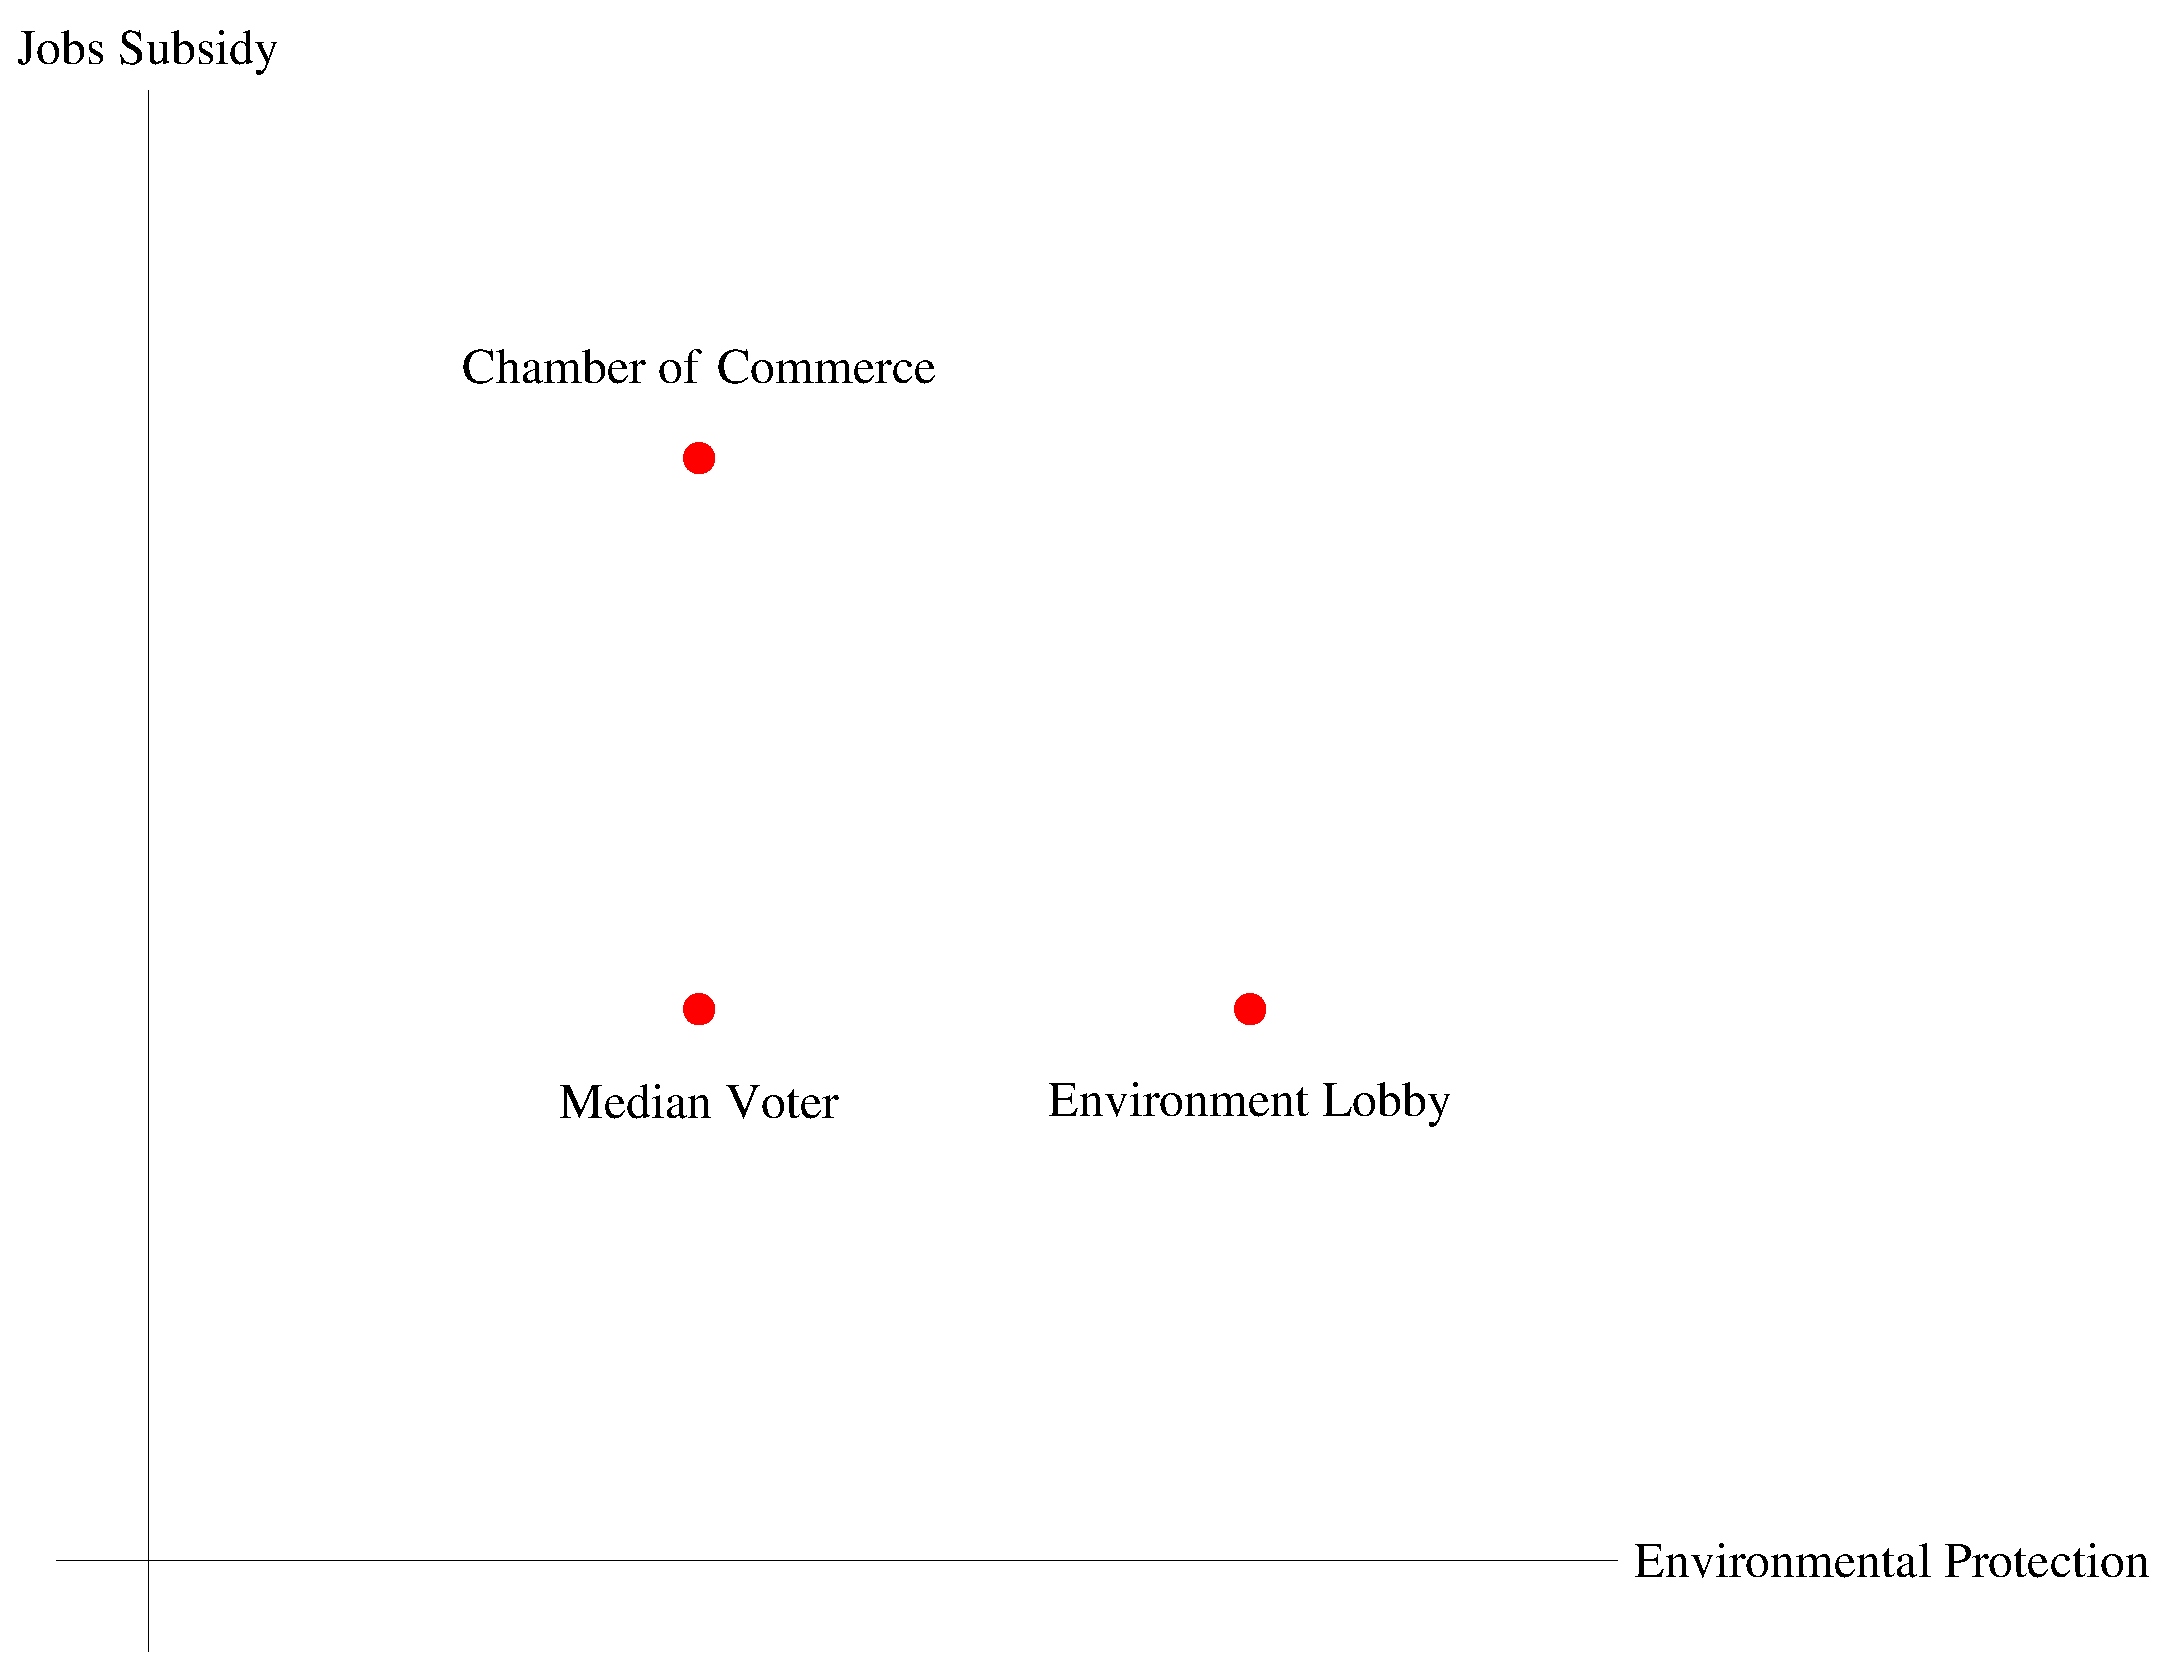
\includegraphics[width=0.8\textwidth]{./i/ExpertsEnvironment.eps}
\end{frame}

\begin{frame}{Example 2: Financial Advisers}
		\begin{itemize}
			\item Consumer seeks to invest her retirement savings in two mutual funds $A$ and $B$ and risk-free treasuries.
			\item Policy is a combination of:
				\begin{itemize}
					\item A choice of how much in total to invest in the equity funds
					\item How to divide that amount between the two funds
				\end{itemize} \pause
			\item Two experts provide advice:
				\begin{itemize}
					\item Fund A Representative
					\item Fund B Representative
				\end{itemize}
				\pause
			\item Can the consumer discover her optimal portfolio?
		\end{itemize}

\end{frame}

\begin{frame}{Investment Example}
	\centering \includegraphics<1>[width=0.8\textwidth]{./i/Experts3.eps}
\end{frame}

\begin{frame}
\begin{card}{Research Question:}
	Can competition between biased information sources lead to more informed consumers?
\end{card}
\end{frame}

\begin{frame}{Theory Summary}
	\begin{itemize}
		\item With just one sender and misaligned preferences, there is no full-revelation
		\item Additional senders in one dimension leads to possibility of more information transfer, but not robust
		\item With multiple dimensions, competition between senders generically leads to existence of fully revealing equilibrium.
	\end{itemize}
\end{frame}


\subsection{Theory}
\begin{frame}{Theory}
	\begin{center}
		\begin{tabular}{ccc} \toprule
		Policy Dimension	&  One-Sender   & Multiple-Senders   \\  \midrule
		Univariate			&  \showOn{Crawford \& Sobel}{2}{1} &   \color{white}{Krishna \& Morgan} \\
		Multivariate		&	\color{white}{Crawford \& Sobel} &	\color{white}{Battaglini}	\\  \bottomrule
		\end{tabular}
	\end{center}
\end{frame}

\begin{frame}{Crawford-Sobel Example}
	\begin{center}\includegraphics<1>[width=1.0\textwidth]{./i/CSexample-1.eps}\includegraphics<2>[width=1.0\textwidth]{./i/CSexample-2.eps}\includegraphics<3>[width=1.0\textwidth]{./i/CSexample-3.eps}\includegraphics<4>[width=1.0\textwidth]{./i/CSexample-4.eps}\includegraphics<5>[width=1.0\textwidth]{./i/CSexample-5.eps}\includegraphics<6>[width=1.0\textwidth]{./i/CSexample-6.eps}\includegraphics<7>[width=1.0\textwidth]{./i/CSexample-7.eps}\includegraphics<8>[width=1.0\textwidth]{./i/CSexample-8.eps}\includegraphics<9>[width=1.0\textwidth]{./i/CSexample-9.eps}\includegraphics<10>[width=1.0\textwidth]{./i/CSexample-10.eps}\includegraphics<11>[width=1.0\textwidth]{./i/CSexample-11.eps}\includegraphics<12>[width=1.0\textwidth]{./i/CSexample-12.eps}\includegraphics<13>[width=1.0\textwidth]{./i/CSexample-13.eps}\includegraphics<14>[width=1.0\textwidth]{./i/CSexample-13.eps}
	\end{center}

	\only<1-2>{State realized}
	\only<3-4>{Sender $X$ has optimal point $b$ to right of $\theta$}
	\only<5-6>{Sender $X$ sends a message $x$}
	\only<7-8>{Receiver $Z$ makes a choice $z$, optimal point of $\theta$}
	\only<9>{Sender sees state, could reveal truth with $x$.}
	\only<10>{In which case the Receiver chooses their best point}
	\only<11>{Not Equilibrium, as now the sender exaggerates...}
	\only<12>{...to which the receiver reacts...}
	\only<13>{...and on...}
	\only<14>{...and on.}
\end{frame}

\begin{frame}{Theory}
	\begin{center}
		\begin{tabular}{ccc} \toprule
		Policy Dimension	&  One-Sender   & Multiple-Senders   \\  \midrule
		Univariate			&  Crawford \& Sobel &   \showOn{Krishna \& Morgan}{2}{1} \\
		Multivariate		& \color{white}{Crawford \& Sobel}  &	\color{white}{Battaglini} \\  \bottomrule
		\end{tabular}
	\end{center}
\end{frame}

\begin{frame}{Krishna-Morgan, Misaligned Senders}
	\begin{center}
		\includegraphics<1>[width=1.0\textwidth]{./i/GJexample-1.eps}\includegraphics<2>[width=1.0\textwidth]{./i/GJexample-2.eps}\includegraphics<3>[width=1.0\textwidth]{./i/GJexample-3.eps}\includegraphics<4>[width=1.0\textwidth]{./i/GJexample-4.eps}\includegraphics<5>[width=1.0\textwidth]{./i/GJexample-5.eps}\includegraphics<6->[width=1.0\textwidth]{./i/GJexample-6.eps}
	\end{center}
	
	\only<1>{State realized}\only<2>{Two advisers either side of you}\only<3>{Two messages, one from each adviser}\only<4>{Equilibrium: if they agree, choose their recommendation}\only<5-6>{Equilibrium: if they disagree, punish}\only<7>{Non-robust: small errors? non-credible threat?}
\end{frame}



\begin{frame}{Theory}
	\begin{center}
		\begin{tabular}{ccc} \toprule
		Policy Dimension	&  One-Sender   & Multiple-Senders   \\  \midrule
		Univariate			&  Crawford \& Sobel &   Krishna \& Morgan \\
		Multivariate		&  Crawford \& Sobel &	\showOn{Battaglini}{2}{1}	\\  \bottomrule
		\end{tabular}
	\end{center}
\end{frame}

\begin{frame}{Multidimensional, Multi-Sender Example}
	\begin{center}
		\includegraphics<1>[width=0.8\textwidth]{./i/SenderPrefs0.eps}\includegraphics<2>[width=0.8\textwidth]{./i/SenderPrefs3-1.eps}\includegraphics<3>[width=0.8\textwidth]{./i/SenderPrefs3-2.eps} \includegraphics<4>[width=0.8\textwidth]{./i/SenderPrefs3-3.eps}\includegraphics<5>[width=0.8\textwidth]{./i/SenderPrefs3-4.eps}\includegraphics<6>[width=0.8\textwidth]{./i/SenderPrefs3-2.eps}\includegraphics<7>[width=0.8\textwidth]{./i/ReceiverPrefs1.eps}\includegraphics<8>[width=0.8\textwidth]{./i/ReceiverPrefs2.eps}\includegraphics<9>[width=0.8\textwidth]{./i/Equilib1-3.eps}\includegraphics<10>[width=0.8\textwidth]{./i/Equilib1-1.eps}\includegraphics<11>[width=0.8\textwidth]{./i/Equilib1-2.eps}\includegraphics<12>[width=0.8\textwidth]{./i/Equilib1-3.eps}\includegraphics<13>[width=0.8\textwidth]{./i/Equilib2-3.eps}\includegraphics<14>[width=0.8\textwidth]{./i/Equilib2-1.eps}\includegraphics<15>[width=0.8\textwidth]{./i/Equilib2-2.eps}\includegraphics<16>[width=0.8\textwidth]{./i/Equilib2-3.eps}
	\end{center}
\end{frame}
\begin{frame}{Alternative Solution}
	\begin{itemize}
		\item Suppose the players exaggerate in the direction of their bias:
		$$\mathbf{x}(\boldsymbol{\theta})=\boldsymbol{\theta}+k_x \cdot \boldsymbol{\delta}_X $$
		$$\mathbf{y}(\boldsymbol{\theta})=\boldsymbol{\theta}+k_y \cdot \boldsymbol{\delta}_Y $$
		where $k_X$ and $k_Y$ represent the degree of exaggeration.\pause
		\item Eliminating the unknown state $\boldsymbol{\theta}$ we get:
		$$\mathbf{y}(\boldsymbol{\theta})-\mathbf{x}(\boldsymbol{\theta})=k_Y \cdot \boldsymbol{\delta}_Y-k_X \cdot \boldsymbol{\delta}_X$$ \pause
		\item But only $k_X$ and $k_Y$ are unknowns---2 unknowns in $n\geq2$ equations.\pause
		%\item So the receiver makes a choice:
		%		$$\mathbf{x}-k_x\left(\mathbf{y}-\mathbf{x};\boldsymbol{\delta}_X,\boldsymbol{\delta}_Y\right)\cdot\boldsymbol{\delta}_X $$
		%

	\end{itemize}
\end{frame}
\begin{frame}{Alternative Solution Example}
	\begin{itemize}
		\item Consider the case where:
		$$\boldsymbol{\delta}_X=\left( \begin{array}{c} -1 \\ 1 \end{array} \right)\text{ and } \boldsymbol{\delta}_Y=\left( \begin{array}{c} 1 \\ 1\end{array}\right)$$\pause
		\item We therefore know that:
		$$\left(\begin{array}{r} y_1-x_1 \\ y_2-x_2 \end{array}\right) =\left(\begin{array}{r} k_y+k_x \\ k_y-k_x \end{array}\right)$$\pause
		\item So the difference in the two recommendations tells us
		\begin{enumerate}
			\item The sum of their exaggerations
			\item The difference in the exaggerations.
		\end{enumerate}
	\end{itemize}
\end{frame}
\begin{frame}{Theory}
	\begin{center}
		\begin{tabular}{ccc} \toprule
		Policy Dimension	&  One-Sender   & Multiple-Senders   \\  \midrule
		Univariate			& No Full Revelation &   Non-Robust Equilibria \\
		Multivariate		&  No Full Revelation &	Full Revelation	\\  \bottomrule
		\end{tabular}
	\end{center}
\end{frame}


\subsection{Experiment}
\begin{frame}{How do we implement this in the lab?}
	\begin{itemize}
		\item Two dimensions.
		\item 3 subjects in a group:
		\begin{itemize}
			\item 2 Senders with differing biases
			\begin{itemize}
				\item Each sends a message in the plane
			\end{itemize}
			\item 1 Receiver
			\begin{itemize}
				\item Given the two messages, chooses a point in the plane.
			\end{itemize}
		\end{itemize}
		\item Pay the subjects \$20 if chosen point is their best location
		\item Payoffs decreasing in the distance from chosen point
	\end{itemize}
\end{frame}

\begin{frame}{Problems with boundedness}
	\centering \includegraphics<1>[width=0.8\textwidth]{./i/Bounded1.eps}\includegraphics<2>[width=0.8\textwidth]{./i/Bounded.eps}\includegraphics<3>[width=0.8\textwidth]{./i/Bounded2.eps}
\end{frame}

\begin{frame}{Solution to boundedness}
	\begin{itemize}
		\item We use two clocks as the state space, one for each dimension
		\item We relocate the Euclidean plane to the surface of the unit sphere
			\begin{itemize}
				\item No boundaries to consider
				\item Can use a non-modal uniform distribution
			\end{itemize}
	\end{itemize}
\end{frame}

\begin{frame}{General Design}
	\begin{itemize}
		\item Between subject
		\begin{itemize}
			\item Treatment consist of an orientation
			% \item Randomize axes and sender identities
		\end{itemize}
		\item Fifteen rounds with role switching every 5: $X$, $Y$ and $Z$
		\item Last five rounds everyone is the receiver $Z$
		\begin{itemize}
			\item Generate extra data for receivers
			\item Remove other-regarding concerns
		\end{itemize}
	\end{itemize}
\end{frame}

\begin{frame}{Preferences}
	\begin{itemize}
		\item Every subject in the game is told their best point
			\begin{itemize}
				\item Receiver is the true state
				\item Senders are the true state plus their bias
			\end{itemize}
		\item Monetary payoffs are given by:
		$$\min\left\{ \$5,\$20-\$8\frac{\sqrt{\textrm{(\small Distance Best \ensuremath{1})}^{2}+\textrm{(\small Distance Best \ensuremath{2})}^{2}}}{45^{\circ}}\right\}$$
		\item Final payment is two random rounds.
	\end{itemize}
\end{frame}

\begin{frame}{Treatment\only<1>{---$R(0)$}\only<2>{---$R(1)$}}
	\centering \includegraphics<1>[width=0.8\textwidth]{./i/TreatmentAA.eps}\includegraphics<2>[width=0.8\textwidth]{./i/TreatmentSR.eps}
	% \centering \includegraphics<2>[width=0.8\textwidth]{./i/TreatmentAR.eps}
\end{frame}

\begin{frame}{Round Details}
	\begin{center}
	\centering \includegraphics<1>[width=0.8\textwidth]{./i/Timeline1.eps}\includegraphics<2>[width=0.8\textwidth]{./i/Timeline2.eps}\includegraphics<3>[width=0.8\textwidth]{./i/Timeline3.eps}\includegraphics<4>[width=0.8\textwidth]{./i/Timeline.eps}

	\end{center}

	\begin{enumerate}
		\setcounter{enumi}{-1}
		\item States $\theta_1$ and $\theta_1$ drawn uniformly from $\left\{1,\ldots,360\right\}$
		\item \showOn{Senders $X$ and $Y$ observe $\boldsymbol{\theta}$, choose messages $\mathbf{x}(\boldsymbol{\theta})$ and $\mathbf{y}(\boldsymbol{\theta})$}{2-4}{1}
		\item \showOn{Receiver observes $\mathbf{x}$ and $\mathbf{y}$, makes final choice $\mathbf{z}(\mathbf{x},\mathbf{y})$}{3-4}{1-2}
		\item \showOn{Feedback on outcomes}{4}{1-3}
	\end{enumerate}
\end{frame}

\begin{frame}{}
	What does the interface look like?

	(if we have time!)
\end{frame}


\subsection{Results}
\begin{frame}{}
Results...
\end{frame}
\begin{frame}{Message Exaggeration: $R(0)$}
	\centering \includegraphics<1>[width=0.7\textwidth]{./i/MessagesAAc_All.eps}\includegraphics<2>[width=0.7\textwidth]{./i/MessagesAAc_Last5.eps}\includegraphics<3>[width=0.7\textwidth]{./i/MessagesAAc_BR_All.eps}
\end{frame}

\begin{frame}{Message Exaggeration: $R(1)$}
	\centering \includegraphics<1>[width=0.7\textwidth]{./i/MessagesSRc_All.eps}\includegraphics<2>[width=0.7\textwidth]{./i/MessagesSRc_Last5.eps}\includegraphics<3>[width=0.7\textwidth]{./i/MessagesSRc_BR_All.eps}
\end{frame}

\begin{frame}{Message Exaggeration: $R(0.6)$}
	\centering \includegraphics<1>[width=0.7\textwidth]{./i/MessagesARc_All.eps}\includegraphics<2>[width=0.7\textwidth]{./i/MessagesARc_Last5.eps}\includegraphics<3>[width=0.7\textwidth]{./i/MessagesARc_BR_All.eps}
\end{frame}

% \begin{frame}{Message Exaggeration: Perfectly Aligned Senders}
% 	\centering \includegraphics<1>[width=0.8\textwidth]{./i/MessagesUAc_All.eps}
% 	\centering \includegraphics<2>[width=0.8\textwidth]{./i/MessagesUAc_Last5.eps}
% 	\centering \includegraphics<3>[width=0.8\textwidth]{./i/MessagesUAc_BR_All.eps}
% \end{frame}

% \begin{frame}{Message Exaggeration: One Sender}
% 	\centering \includegraphics<1>[width=0.8\textwidth]{./i/Messages1Sc_All.eps}
% 	\centering \includegraphics<2>[width=0.8\textwidth]{./i/Messages1Sc_Last5.eps}
% 	\centering \includegraphics<3>[width=0.8\textwidth]{./i/Messages1Sc_BR_All.eps}
% \end{frame}

\begin{frame}{Summary of message behavior}
	\begin{itemize}
		\item In both treatments senders provide messages close to the ray defined by their bias
		\item Slightly more exaggeration in the direction of opposition in the rotated environment
	\end{itemize}
\end{frame}

\begin{frame}{Extraction of Information, Payment CDFs}
	\begin{center}
        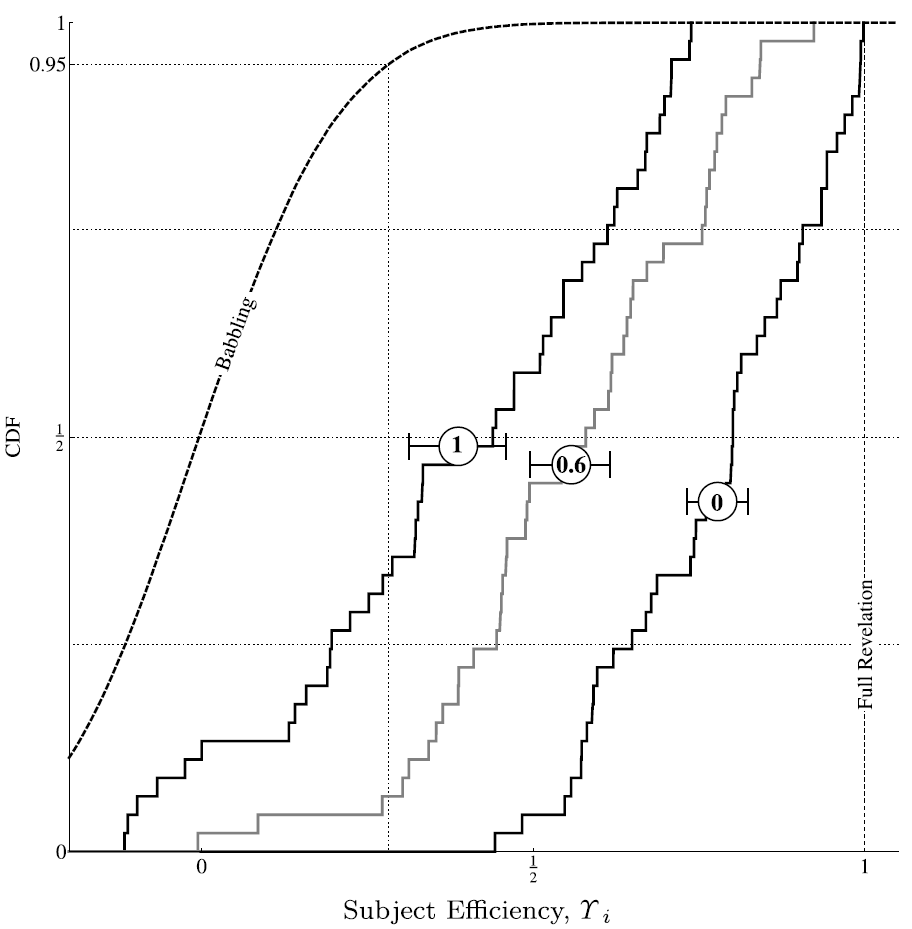
\includegraphics[width=0.6\textwidth]{./i/vw_SubEff1.png}
	\end{center}
\end{frame}
\begin{frame}{Extraction of Information, Counter-factual Payment CDFs}
	\begin{center}
        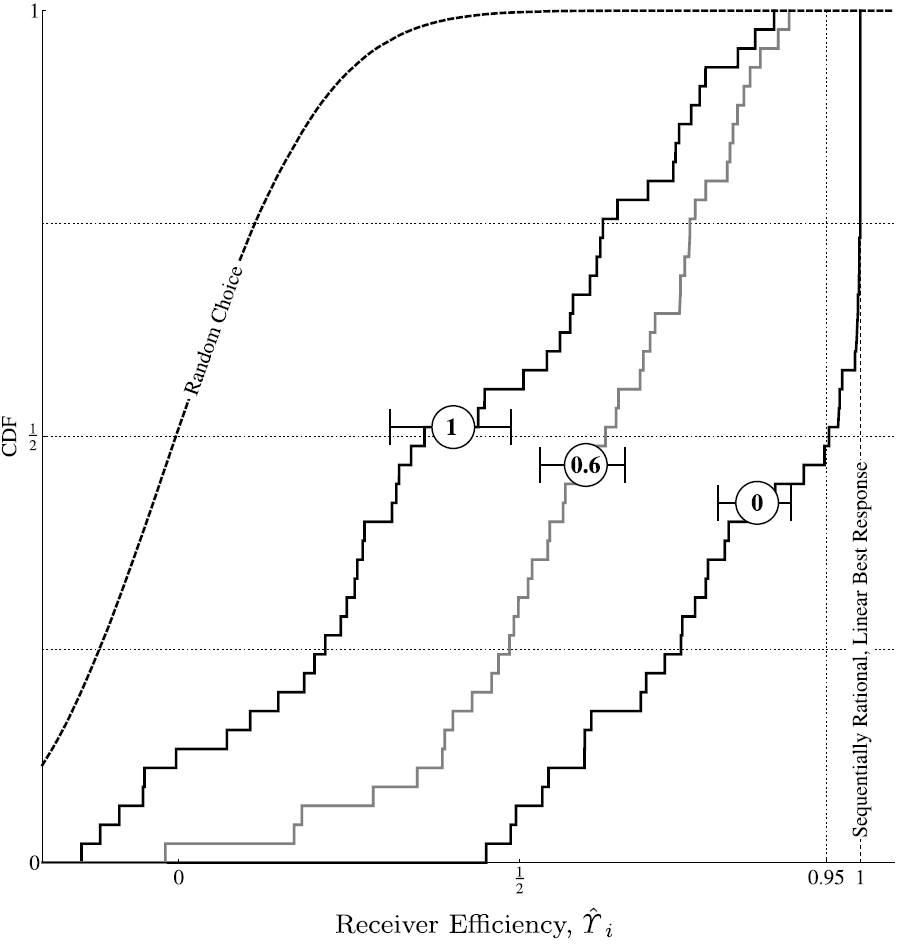
\includegraphics[width=0.6\textwidth]{./i/vw_SubEff2.png}
	\end{center}
\end{frame}

\begin{frame}{Receiver strategies---Estimates}
	\begin{center}
		\begin{tabular}{lccccc}\hline
		 & \multicolumn{2}{c}{Theory} & & \multicolumn{2}{c}{Estimated}\\\cline{2-3}\cline{5-6}
		Treatment & $\alpha$ & $\beta$  & & $\hat{\alpha}$ & $\hat{\beta}$ \\ \hline
			AA  & 1.00 & 0.00 & &0.85 & -0.02 \\
			    & 0.00 & 0.00 & &0.15 & -0.08\\
			SR  & 0.50 & -0.50 & &0.42 &-0.09 \\
			    & 0.50 & 0.50 & &0.56 &-0.03 \\
			AR  & 0.74 & -0.44 & &0.67 &-0.05 \\
			    & 0.26 & 0.44 &  &0.38 &-0.05 \\ \hline
		\end{tabular}
	\end{center}
	\begin{itemize}
		\item Estimate the relationship:
			$$z^1_{it}=\alpha^1 x^1_{it}+(1-\alpha^1)y^1_{it} +\beta^1(x^2_{it}-y^2_{it}) +\epsilon^1_{it}$$
			$$z^2_{it}=\alpha^2 x^2_{it}+(1-\alpha^2)y^2_{it} +\beta^2(x^1_{it}-y^1_{it}) +\epsilon^2_{it}$$
	\end{itemize}
\end{frame}


\begin{frame}{Receiver strategies}
	\begin{itemize}
		\item Look at the dimension $i$ on which the subjects are opposed.
		\item The recommendations $x_i$ and $y_i$ should lie either side of the true state\pause
		\item Whereabouts do senders locate on the interval between these two messages:
		$$\alpha_i=\frac{z_i-x_i}{y_i-x_i} $$\pause
		\item If the biases are symmetrically opposed, locate toward the sender you trust more
	\end{itemize}
\end{frame}

\begin{frame}{Location of decision between opposed senders}
	\centering 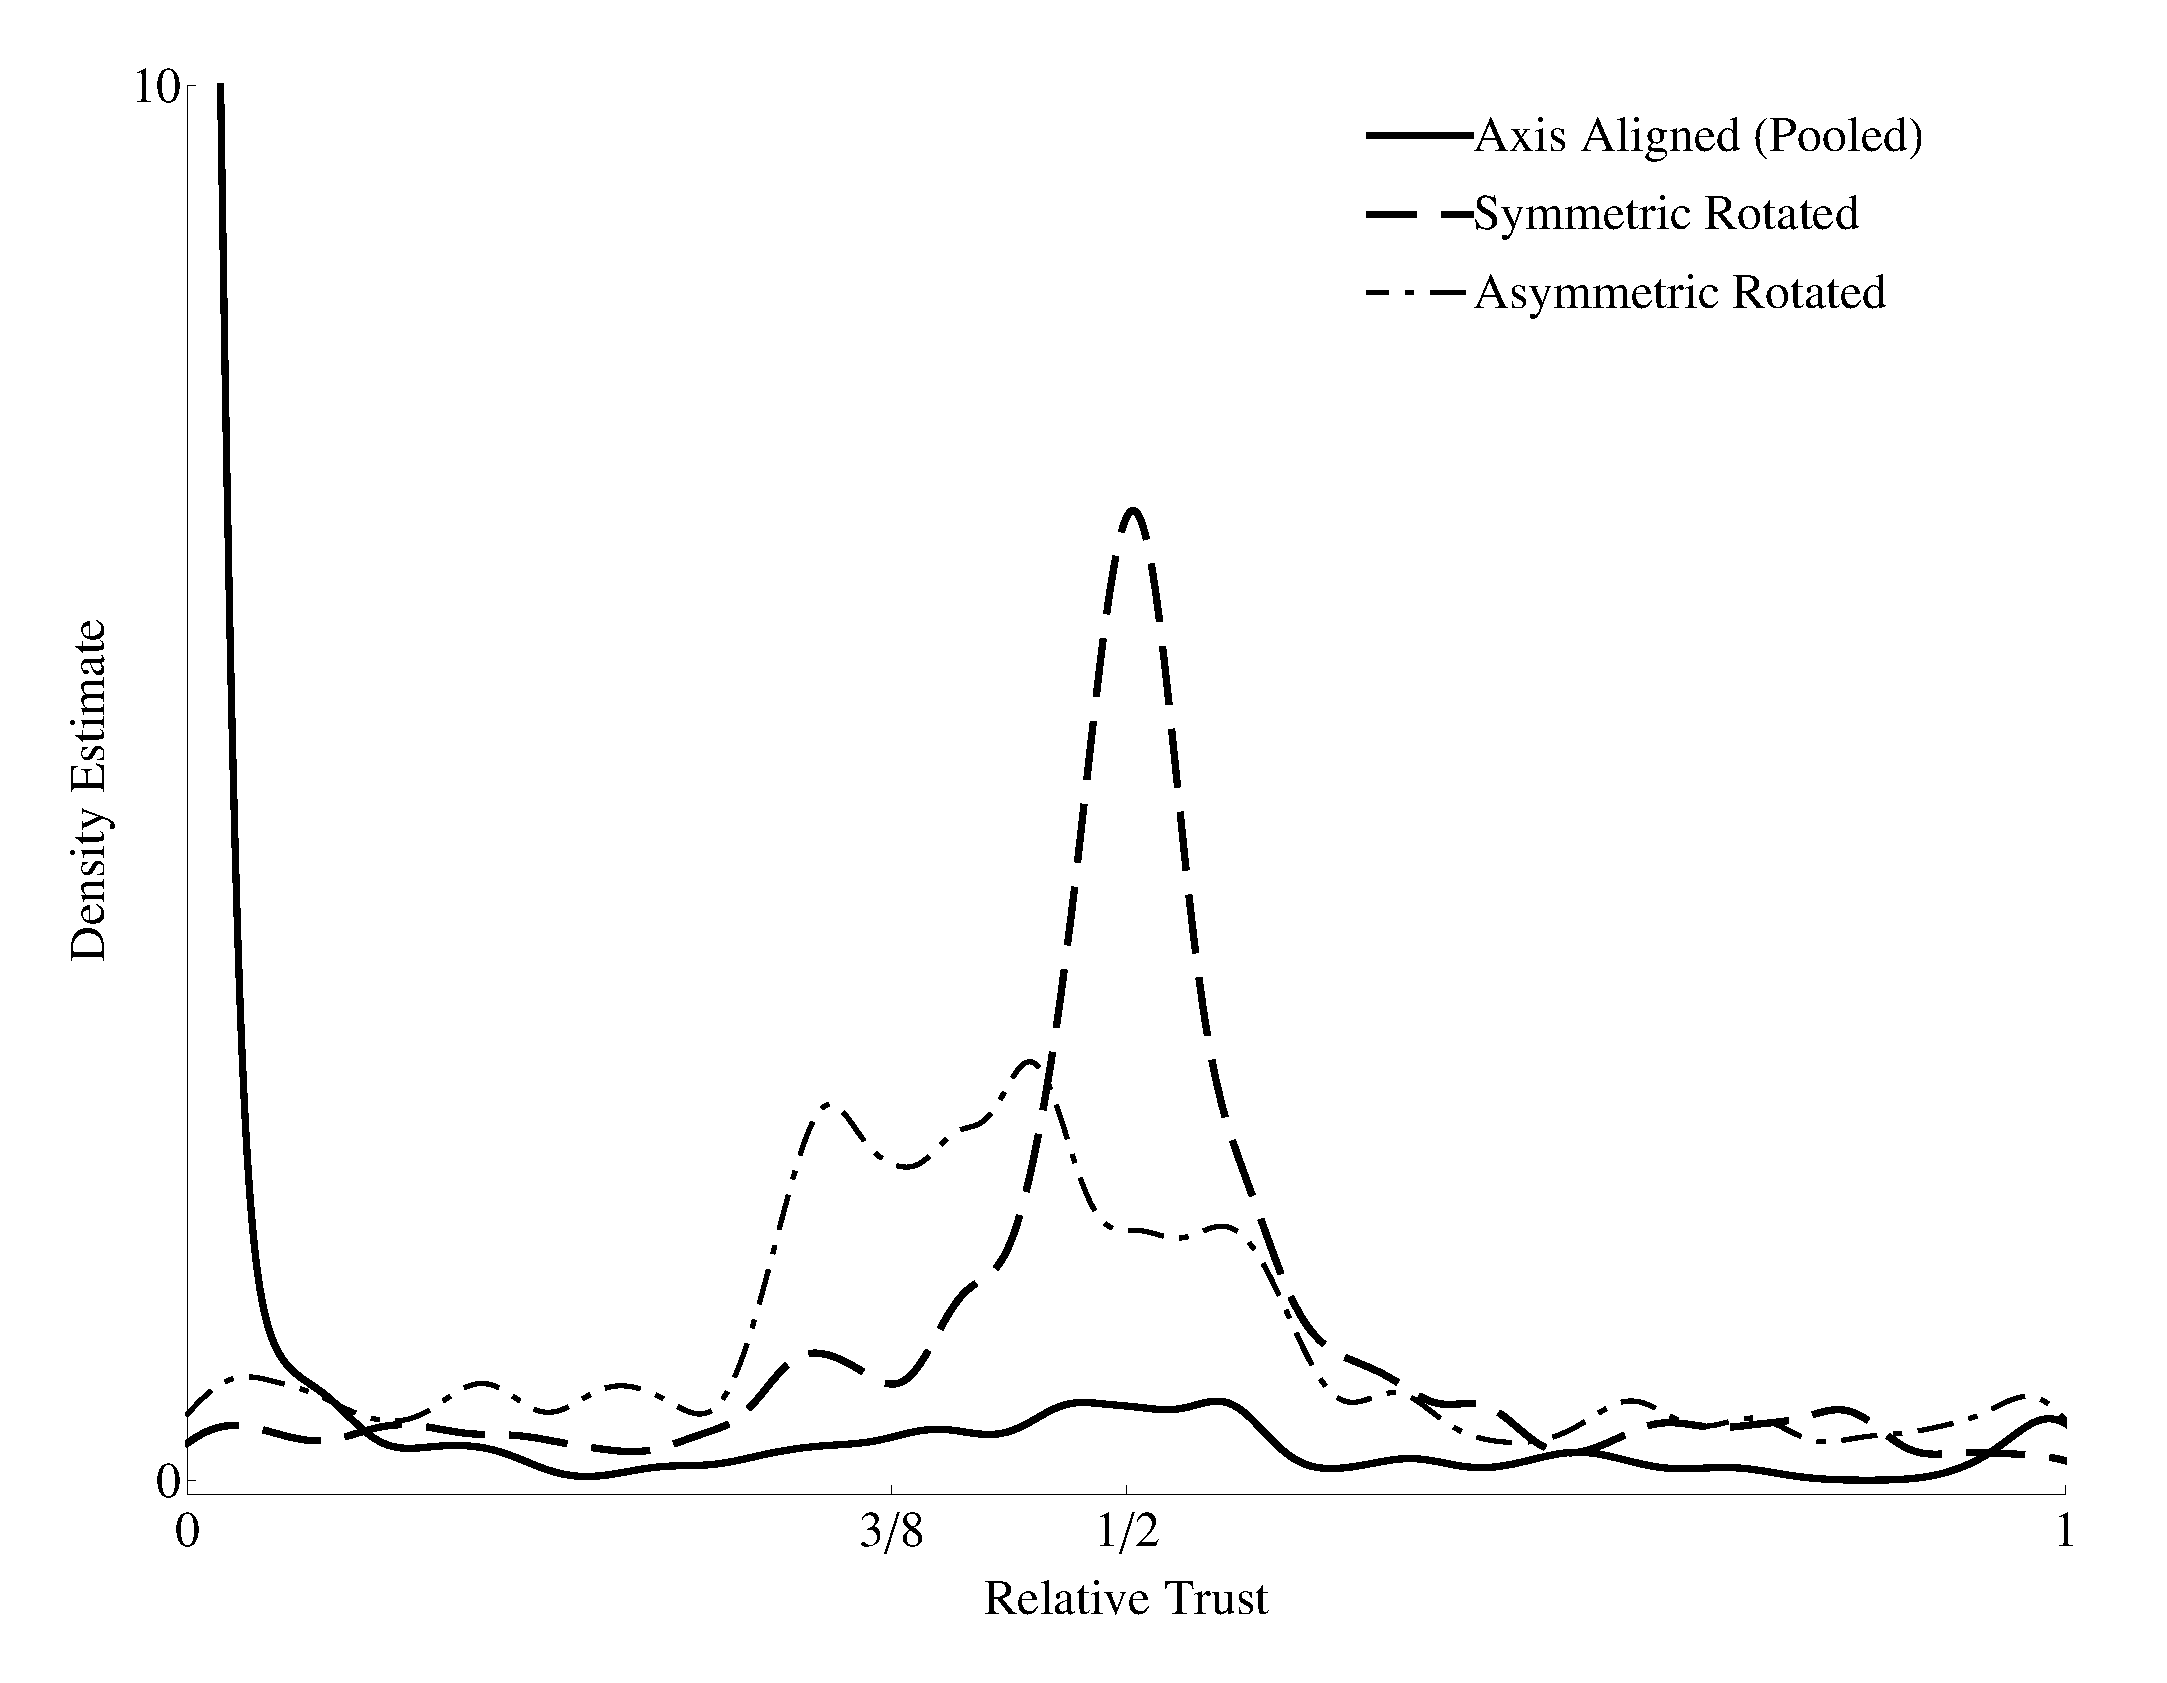
\includegraphics[width=0.8\textwidth]{./i/OpposedSenderTrust_KernelM.eps}
\end{frame}

\begin{frame}{Unidimensional Response---$R(0)$}
	\centering 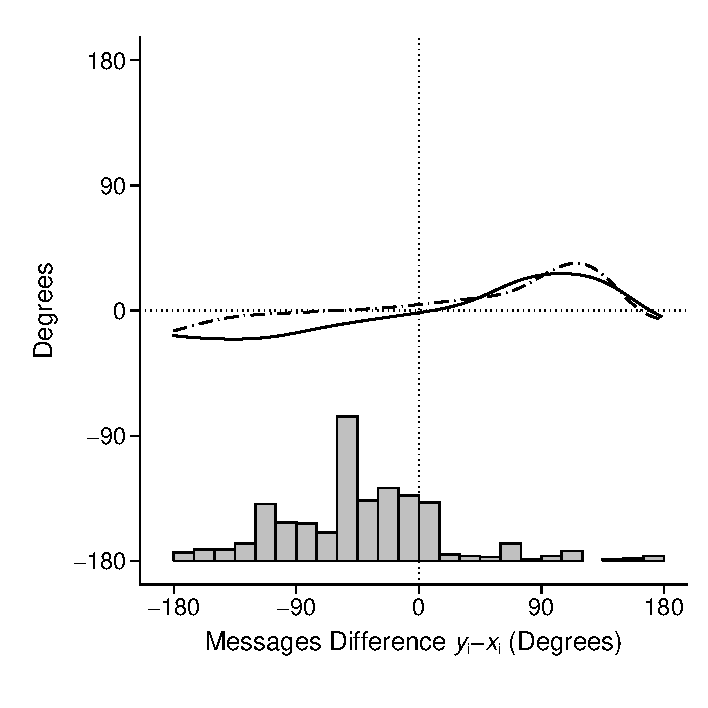
\includegraphics[width=0.8\textwidth]{./i/ConditionalChoiceWHist_AA_2.eps}
\end{frame}
\begin{frame}{Unidimensional Response---$R(1)$ (Opposed)}
	\centering 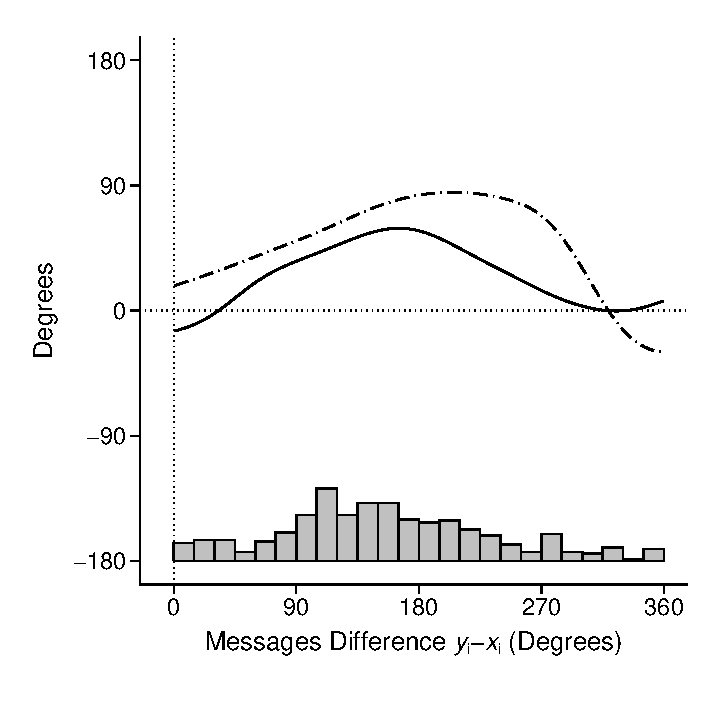
\includegraphics[width=0.8\textwidth]{./i/ConditionalChoiceWHist_SR_1.eps}
\end{frame}

\begin{frame}{Unidimensional Response---$R(1)$ (Aligned)}
	\centering 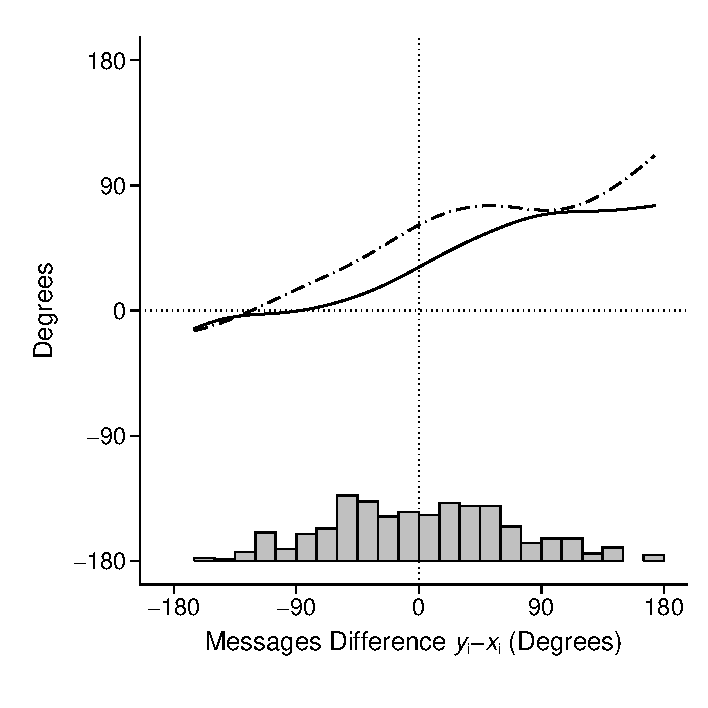
\includegraphics[width=0.8\textwidth]{./i/ConditionalChoiceWHist_SR_2.eps}
\end{frame}

\begin{frame}{Location of decision between opposed senders}
	\begin{itemize}
		\item But in the rotated treatments the equilibrium requires receivers to react more to the recommendations of those who seem trustworthy in the other dimension
		\item We regress the point in between the opposed signals $\alpha_{it}$ on which sender seemed more trustworthy
		\item Find no significant effects \pause
		\item {\bf Conclusion: receivers only react to \emph{ex ante} trustworthiness, not to the information contained in the signals}
	\end{itemize}
\end{frame}

\begin{frame}{Summary}
	\begin{itemize}
		\item Simple graphical implementation of Battaglini (2002)
		\item Very little \emph{Honest} revelation by senders
		\item Subjects are much more successful at extracting information in the $R(0)$ environment
		\item Once biases become more complex receivers do not extract information optimally, despite large potential gains
		\item Subjects only react to \emph{ex ante} trust in senders
	\end{itemize}
\end{frame}

\section{Repeated Sender Receiver}
\title{Information Relationships}
\author{$\begin{array}{cc} \text{Alistair Wilson } & \text{Emanuel Vespa
}
\\ \text{\small Pittsburgh} & \text{\small UCSB }\end{array}$  }


\maketitle

\subsection{Intro}
\begin{frame}{Two main motivating questions}
    \begin{itemize}
        \item \textbf{Specific:} Many information transmission problems have inefficient
        outcomes in static setting; natural to ask: 
            \begin{itemize}
            \item Does repetition lead to more information revelation?\bigskip{}
            \end{itemize}
        \item \textbf{General:} Selection in repeated games:
            \begin{itemize}
            \item Can we reduce the folk theorem's predictive indeterminacy?
            \end{itemize}
    \end{itemize}
\end{frame}

\begin{frame}{Question 1: Repetition and Information Transmission}
    \begin{itemize}
    \item Important topic in economics, accounting, finance and political science
    \item A large literature has examined one-shot strategic information transmission
        \begin{itemize}
        \item Theoretically
        \item Experimentally
        \end{itemize}
    \item Though the literature has focused on one-shot, many applied situations
    are repeated, ongoing relationships
    \end{itemize}
\end{frame}

\begin{frame}{Question 2: Reduce Indeterminacy}
    \begin{itemize}
        \item Beyond a specific interest in repeated information transmission, the
        environment offers a test-bed to examine repeated game strategies\bigskip{}
        \item Folk theorems, though theoretically elegant are essentially negative
        results for prediction
        \item Can we reduce the indeterminacy by appealing to behavioral regularities
        over selections?
            \begin{itemize}
                \item Current literature suggest strategic uncertainty is important for
                coordination in PD games
            \end{itemize}
    \end{itemize}
\end{frame}

\begin{frame}{Question 2: Reduce Indeterminacy}
Experimental evidence on selection largely uses PD stage games:
    \begin{enumerate}
        \item Symmetric
        \item Efficient outcome is unique
        \item Efficient play supported by:
            \begin{enumerate}
            \item ``Simple'' on-path play
            \item Harshest punishments are also ``simple''
            \end{enumerate}
    \end{enumerate}
Coordination issues: Which punishments are used to support the efficient
outcome?

\end{frame}

\begin{frame}{Question 2: Reduce Indeterminacy}
Our baseline environment:
    \begin{enumerate}
        \item Asymmetric
        \item Many efficient outcomes
        \item Efficient play represents a tradeoff
            \begin{enumerate}
            \item Efficient outcomes with ``simple'' on-path play require complex punishments
            \item Simple supporting punishents require greater coordination on the path
            \end{enumerate}
    \end{enumerate}
Coordination issues: Which on-path play? Which punishments? Is the
combination an equilibrium?
\end{frame}

\begin{frame}{Question 2: Reduce Indeterminacy}
    \begin{itemize}
        \item Use experimental treatments that vary which efficient outcomes can
        be supported with which punishments to understand selection
        \item Find that ``simple'' punishments are focal
        \item But ``simple'' punishments not sufficient without strong coordination
        devices
            \begin{itemize}
                \item Also need the efficient outcomes supported by Nash reversion to have
                ``simple'' on-path play
            \end{itemize}
    \end{itemize}
\end{frame}

\begin{frame}{Game Set-up}
    \begin{itemize}
    \item Minimally simple:
        \begin{itemize}
            \item \textbf{Two players}: a sender and a receiver
            \item \textbf{Two states}: good or bad
            \item \textbf{Two messages}: natural language framing to states
            \item \textbf{Three actions:} two risky options connected to states, and
            a safe option
        \end{itemize}
    \end{itemize}
\end{frame}

\begin{frame}{Payoffs}
	\begin{center}%
		\begin{tabular}{c|cc|c|c|}
		\multicolumn{1}{c}{} &  & \multicolumn{1}{c}{} & \multicolumn{2}{c}{State, $\theta$} \\ 
		\cline{4-5} 
		\multicolumn{1}{c}{} &  & \multicolumn{1}{c}{} & \multicolumn{1}{c}{Good} & \multicolumn{1}{c}{Bad} \\ 
		\cline{4-5} 
		Action, &  & Full & (1,1) & (1,0) \\ 
		\cline{4-5} 
		$a$ &  & Partial & ($\frac{1}{3},\frac{2}{3}$) & ($\frac{1}{3},\frac{2}{3}$) \\ 
		\cline{4-5} 
		 &  & None & (0,0) & (0,1) \\ 
		\cline{4-5} 
		\multicolumn{3}{c}{\emph{(Sender,Receiver)}} & \multicolumn{1}{c}{} & \multicolumn{1}{c}{} \\ 
		\end{tabular}
	\end{center}
	
	\begin{itemize}
		\item \emph{Good} and \emph{Bad} are selected independently with equal probability
		\item Sender observes state, sends either ``Invest'' or ``Don't Invest''
	message
		\begin{itemize}
			\item Always prefers full investment
			\item Partial investment is the best option for an uninformed receiver
		\end{itemize}
	\end{itemize}
\end{frame}


\begin{frame}{Efficiency state and Distribution state distinction}
\begin{center}%
    \begin{tabular}{c|cc|c|c|}
    \multicolumn{1}{c}{} &  & \multicolumn{1}{c}{} & \multicolumn{2}{c}{State, $\theta$} \\ 
    \cline{4-5} 
    \multicolumn{1}{c}{} &  & \multicolumn{1}{c}{} & \multicolumn{1}{c}{Good} & \multicolumn{1}{c}{Bad} \\ 
    \cline{4-5} 
    Action, &  & Full & (1,1) & (1,0) \\ 
    \cline{4-5} 
    $a$ &  & Partial & ($\frac{1}{3},\frac{2}{3}$) & ($\frac{1}{3},\frac{2}{3}$) \\ 
    \cline{4-5} 
     &  & None & (0,0) & (0,1) \\ 
    \cline{4-5} 
    \multicolumn{3}{c}{\emph{(Sender,Receiver)}} & \multicolumn{1}{c}{} & \multicolumn{1}{c}{} \\ 
    \end{tabular}
\end{center}
    \begin{itemize}
        \item \textbf{\emph{Good}} is the efficiency state, \emph{ex post} agreement
        on the best action
            \begin{itemize}
                \item Pareto ranking: $\text{Full}\succ_{\text{Good}}\text{Partial}\succ_{\text{Good}}\text{None}$
            \end{itemize}
        \item \textbf{\emph{Bad}} is the distributional state, constant sum, \emph{ex
        post} disagreement
            \begin{itemize}
                \item Sender: $\text{Full}\succ_{\text{Bad}}\text{Partial}\succ_{\text{Bad}}\text{None}$ 
                \item Receiver: $\text{None}\succ_{\text{Bad}}\text{Partial}\succ_{\text{Bad}}\text{Full}$ 
            \end{itemize}
    \end{itemize}
\end{frame}

\begin{frame}{Sender's Decision}
    \begin{center}
    \centering \includegraphics<1>[width=\textwidth]{./i/s2_table.eps}
    \end{center}
\end{frame}

\begin{frame}{Receiver's Decision}
\begin{center}
\centering \includegraphics<1>[width=\textwidth]{./i/s4_table.eps}
\end{center}
\end{frame}

\begin{frame}{Main Strategic Tension in the Stage Game}
    \begin{center}%
        \begin{tabular}{c|cc|c|c|}
        \multicolumn{1}{c}{} &  & \multicolumn{1}{c}{} & \multicolumn{2}{c}{State, $\theta$} \\ 
        \cline{4-5} 
        \multicolumn{1}{c}{} &  & \multicolumn{1}{c}{} & \multicolumn{1}{c}{Good} & \multicolumn{1}{c}{Bad} \\ 
        \cline{4-5} 
        Action, &  & Full & (1,1) & (1,0) \\ 
        \cline{4-5} 
        $a$ &  & Partial & ($\frac{1}{3},\frac{2}{3}$) & ($\frac{1}{3},\frac{2}{3}$) \\ 
        \cline{4-5} 
         &  & None & (0,0) & (0,1) \\ 
        \cline{4-5} 
        \multicolumn{3}{c}{\emph{(Sender,Receiver)}} & \multicolumn{1}{c}{} & \multicolumn{1}{c}{} \\ 
        \end{tabular}
    \end{center}
    \begin{itemize}
        \item What to do as a sender when the state is \emph{Bad}?
        \item What to do as a receiver in reaction to \emph{Invest} message?
    \end{itemize}
\end{frame}

\begin{frame}
    \begin{itemize}
        \item ``Simple'' behaviors here:
            \begin{itemize}
                \item \textbf{Sender:} \emph{Honesty} (Reveal State) vs. \emph{Deceive}
                (Always Invest)
                \item \textbf{Receiver:} \emph{Follow Message} vs. \emph{Safe Play} (Always
                Partial)
            \end{itemize}
    \end{itemize}
\end{frame}

\begin{frame}{Repetition}
    \begin{itemize}
        \item We repeat the stage-game so that after every round there is: 
        
            \begin{itemize}
                \item a $\delta$ probability that the game continues for another round
                \item a $1-\delta$ probability that the supergame ends
            \end{itemize}
        \item We use $\delta=\tfrac{3}{4}$ in the sessions\bigskip{}
        \item Precise history becomes common knowledge at end of each round
            \begin{itemize}
                \item Find out if sender lied
                \item Find out what receiver chose
            \end{itemize}
    \end{itemize}
\end{frame}

\begin{frame}{Set of Payoffs and Individually Rational Payoffs}
Focus on payoff space and characterize
the set of individually rational payoffs, what is supportable with
which punishments
\end{frame}

\begin{frame}{Payoff space}
    \begin{center}
    \includegraphics<1>[height=0.8\textheight]{./i/feasibleIRpayoffsBase.eps}
    \end{center}
\end{frame}

\begin{frame}{History-Dependent Strategies}
    \begin{itemize}
    \item With observation of the history in previous rounds
        \begin{itemize}
            \item Can use ``shadow of the future''
            \item Focal conditional event: honesty in previous dealings 
        \end{itemize}
    \item Suppose the receiver wants to fully make use of the provided information
    solely for their own gain
        \begin{itemize}
            \item This implies a required punishment
        \end{itemize}
    \end{itemize}
\end{frame}

\begin{frame}
    \begin{center}
        \includegraphics<1>[height=0.8\textheight]{./i/col_feasibleIRpayoffs5_1.eps}
    \end{center}
Full extraction requires dishonesty to be punished severely
\end{frame}

\begin{frame}{Baseline game}
    \begin{itemize}
        \item The simplest punishment cannot be used to support the simple receiver
        response of fully extracting
        \item More complicated, harsher punishments \textbf{can} support \emph{Full
        Extraction} at $\delta=\tfrac{3}{4}$
        \begin{itemize}
        \item Such punishments are ``complex''
        \end{itemize}
        \item Rather than using a bigger hard-to-weild stick, could also offer a
        better carrot
    \end{itemize}
\end{frame}

\begin{frame}
    \begin{center}
    \includegraphics<1>[height=0.8\textheight]{./i/col_feasibleIRpayoffs5_2.eps}
    \end{center}
\end{frame}

\begin{frame}{Information rents idea}
    \begin{itemize}
    \item Goes back to Baron \& Besanko 1984; Laffont and Tirole 1988
    \item Honesty is not it's own reward in our environment
    \begin{itemize}
    \item The threat of losing one's reputation for honest dealing can only
    be powerful enough to induce good behavior if we punish deviators
    with a very sophisticated response
    \item Unless harsh (and complicated) punishments are used, honesty needs
    to be rewarded on the path
    \end{itemize}
    \item With concavity in the payoffs this is a general feature of these games
    for all $\delta\in(0,1)$
    \end{itemize}
\end{frame}

\begin{frame}{Treatment games }
\begin{itemize}
\item Our treatments vary which efficient outcome can be supported with
`simple' punishments
\item Two treatments in which:
\begin{itemize}
\item Full Extraction can be supported with Nash Reversion
\item Info Rents equilibrium can be supported with Nash Reversion
\end{itemize}
\end{itemize}
\end{frame}

\begin{frame}{Nash=MinMax Treatment 1}
\begin{center}

\begin{tabular}{c|cc|c|c|}
\multicolumn{1}{c}{} &  & \multicolumn{1}{c}{} & \multicolumn{2}{c}{State, $\theta$} \\ 
\cline{4-5} 
\multicolumn{1}{c}{} &  & \multicolumn{1}{c}{} & \multicolumn{1}{c}{Good} & \multicolumn{1}{c}{Bad} \\ 
\cline{4-5} 
Action, &  & Full & (1,1) & (1,0) \\ 
\cline{4-5} 
$a$ &  & Partial & ($\frac{1}{3},\frac{2}{3}$)$\rightarrow$($0,\frac{2}{3}$) & ($\frac{1}{3},\frac{2}{3}$)$\rightarrow$($0,\frac{2}{3}$) \\ 
\cline{4-5} 
 &  & None & (0,0) & (0,1) \\ 
\cline{4-5} 
\multicolumn{3}{c}{\emph{(Sender,Receiver)}} & \multicolumn{1}{c}{} & \multicolumn{1}{c}{} \\ 
\end{tabular}
\begin{itemize}
\item Shift the sender's payoff under Nash down to the minmax
\begin{itemize}
\item Punishments now hurt more
\end{itemize}
\end{itemize}
\end{center}
\end{frame}

\begin{frame}{Nash=MinMax Treatment 2}
\begin{center}

\begin{tabular}{c|cc|c|c|}
\multicolumn{1}{c}{} &  & \multicolumn{1}{c}{} & \multicolumn{2}{c}{State, $\theta$} \\ 
\cline{4-5} 
\multicolumn{1}{c}{} &  & \multicolumn{1}{c}{} & \multicolumn{1}{c}{Good} & \multicolumn{1}{c}{Bad} \\ 
\cline{4-5} 
Action, &  & Full & (1,1) & (1,0) \\ 
\cline{4-5} 
$a$ &  & Partial & ($\frac{1}{3},\frac{2}{3}$) & ($\frac{1}{3},\frac{2}{3}$) \\ 
\cline{4-5} 
 &  & None & (0,0)$\rightarrow$($\frac{1}{3},0$) & (0,1)$\rightarrow$(\textrm{$\frac{1}{3},$}1) \\ 
\cline{4-5} 
\multicolumn{3}{c}{\emph{(Sender,Receiver)}} & \multicolumn{1}{c}{} & \multicolumn{1}{c}{} \\ 
\end{tabular}
\begin{itemize}
\item Shift the sender's minmax up to the Nash payoff
\begin{itemize}
\item Better on-path payoff under full extraction; deviations less tempting
\end{itemize}
\end{itemize}
\end{center}
\end{frame}

\begin{frame}{Baseline}
\begin{center}
\includegraphics<1>[height=0.8\textheight]{./i/feasibleIRpayoffsBase.eps}\includegraphics<2>[height=0.8\textheight]{./i/feasibleIRpayoffsMinMax.eps}\includegraphics<3>[height=0.8\textheight]{./i/feasibleIRpayoffsNash.eps}
\end{center}

\end{frame}\begin{frame}{Treatment 1 (T1)}
\begin{center}
\includegraphics<1>[height=0.8\textheight]{./i/feasibleIRpayoffsIR1.eps}\includegraphics<2>[height=0.8\textheight]{./i/feasibleIRpayoffsIR1Nash.eps}
\end{center}

\end{frame}
\begin{frame}{Treatment 2 (T2)}
	\begin{center}
\includegraphics<1>[height=0.8\textheight]{./i/feasibleIRpayoffsIR2.eps}\includegraphics<2>[height=0.8\textheight]{./i/feasibleIRpayoffsIR2Nash.eps}
	\end{center}
\end{frame}

\begin{frame}{Our Experiment}
\begin{itemize}
\item Nine treatment environments in total

\begin{itemize}
\item Three sessions per treatment
\item 20 Supergames per session
\item 16 participants per session
\item Paid for three random supergames
\end{itemize}
\item First consider:

\begin{enumerate}
\item \textbf{Baseline}:
\begin{itemize}
\item Info Rents eq. supported with Babbling
\item Full Extraction supported with MinMax
\end{itemize}
\item \textbf{Nash=MinMax} treatments: 
\begin{itemize}
\item Any IR efficient outcome supported with Babbling reversion
\item Babbling payoffs in T1 = MinMax payoffs in Baseline
\item Babbling payoffs in T2 = Babbling payoffs in Baseline
\end{itemize}
\end{enumerate}
\end{itemize}
\end{frame}

\begin{frame} 
\begin{center}

\textbf{\textsc{\huge{}Top-Level Results}}{\huge\par}

\end{center}\end{frame}

\begin{frame}{Efficiency }
\begin{center}
Fraction of Good-state rounds with Full Investment minus Fraction
of Good-state rounds with No Investment
\par\end{center}

\begin{center}
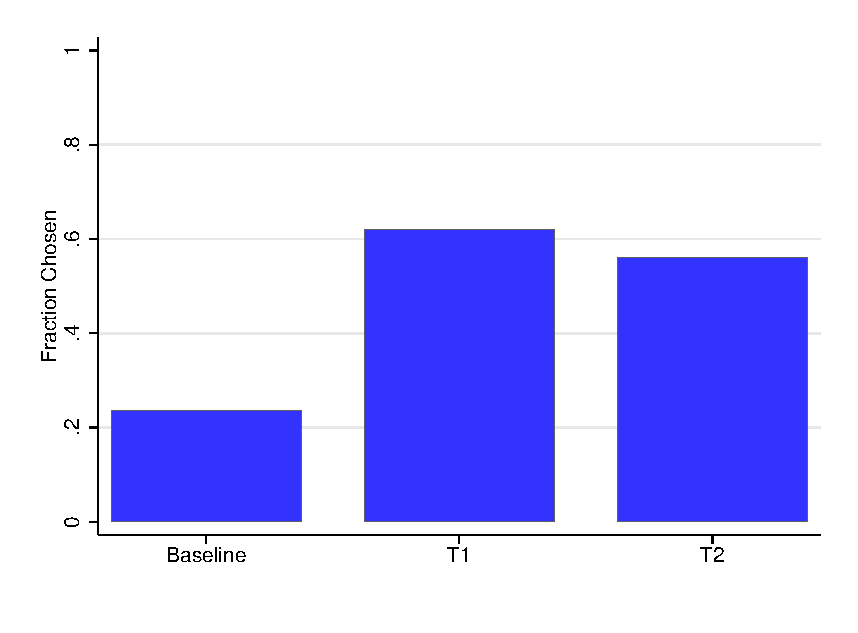
\includegraphics[scale=0.6]{./i/E1_L5A.eps}
\par\end{center}
\end{frame}

\begin{frame}{Result \#1}

Baseline Treatment 
\begin{itemize}
\item Modal behavior is the stage-game equilibrium.
\item Almost all senders lie, claim good state
\item Some evidence for history dependence, but economically small effect
size
\item Low Efficiency\bigskip{}
\end{itemize}
MinMax Treatments 
\begin{itemize}
\item Modal behavior is the efficient outcome with full extraction
\item Senders fully reveal state
\item Efficiency almost triples relative to baseline
\end{itemize}
\end{frame}
\begin{frame}{On-Path Coordination Failures?}
\begin{itemize}
\item Get inefficient outcomes in our baseline; why did they not coordinate
on the information-rents outcome that can be supported by the simple
punishment
\item \textbf{Hypothesis:} Failure in the baseline is due to a coordination
failure over on-path play\bigskip{}
\item \textbf{Chat Treatment}: 
\begin{itemize}
\item Use baseline parameterization
\item Provide a powerful coordination device: pre-play communication
\end{itemize}
\end{itemize}
\end{frame}

\begin{frame}{Chat Treatments}
\begin{itemize}
	\item Supergames 1 to 12, same as baseline
	\item Supergames 13 to 20 have pre-play communication
	\item 16 subjects, in perfect-stranger design for chat
	\item Chat happens before the supergame begins
	\begin{itemize}
		\item Purely coordinative
	\end{itemize}
\end{itemize}
\end{frame}

\begin{frame}{Efficiency }
\begin{center}
Fraction of Good-state rounds with Full Investment minus Fraction
of Good-state rounds with No Investment
\par\end{center}

\begin{center}
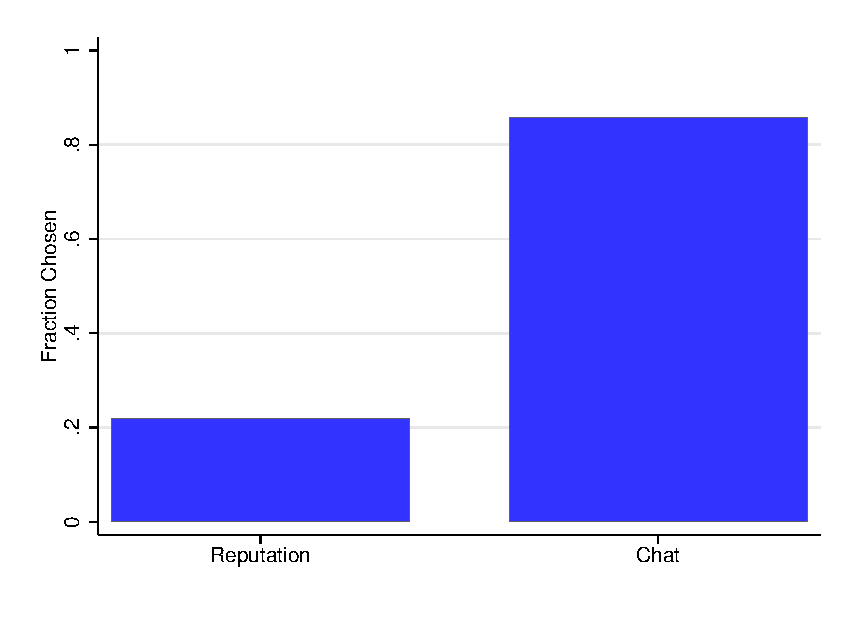
\includegraphics[scale=0.6]{./i/E1_ChatL5A.eps}
\par\end{center}

\end{frame}
\begin{frame}{Chat Examples}

First Chat Supergames:
\begin{quotation}
R(12): hello 

S(3): I'll always give you the correct recommendation if you choose
middle when I say right
\end{quotation}
\end{frame}

\begin{frame}{Chat Examples}

First Chat Supergames:
\begin{quotation}
R(4): no funny business/ :D 

S(11): I'll tell you the actuall direction 

S(11): i know 

R(4): great 

R(4): ill take middle if right 

S(11): You're welcome
\end{quotation}
\end{frame}

\begin{frame}{Chat Examples}

First Chat Supergames:
\begin{quotation}
R(180): I'll trust you until you lie and then it's m,iddles the whole
way out. 

S(18): Hey want to work together on this? 

R(180): If you click right, I'll go middle so we both get something 

S(18): I will tell you all the honest computer decsions if you never
click right 

S(18): instead when i mark right click middle 

S(18): deal? 

R(180): no problem 

R(180): deal
\end{quotation}
\end{frame}

\begin{frame}{Chat Examples}

Early Chat Supergames (14):
\begin{quotation}
R(108): are you going to click honestly? 

S(198): I will give honest reccomendations if you choose middle when
i tell you RIGHT so we both benefit. That wil be my incentive to be
honst 

R(108): cool
\end{quotation}
\end{frame}

\begin{frame}{Chat Examples}

Later Chat Supergames:
\begin{quotation}
S(5): domt go middle 

S(5): {*}DONT 

R(16): in order to get highest profit - i'll trust your recommendations.
for every 'right' the computer chooses, i'll let you trick me once
so that we make equal profit. 

R(16): sound ok? 

S(5): sounds good
\end{quotation}
\end{frame}

\begin{frame}{Chat Examples}

Later Chat Supergames:
\begin{quotation}
R(8): u right i middle 

S(9): when i say L, go L. when i say R, go middle 

R(8): Awesome same thought 
\end{quotation}
\end{frame}

\begin{frame}{Chat}
\begin{itemize}
\item 78\% of chats articulate the information-rents outcome, most the very
first time chat is available
\item Clear that subjects understand this outcome as a possibility, but
cannot coordinate on it
\item Deviations are punished with reversion to babbling
\begin{itemize}
\item Anecdotal evidence in chat logs that agreements are conditional (\textasciitilde 5\%)
\end{itemize}
\end{itemize}
\end{frame}

\begin{frame}
{\Large Result \#2:}
\begin{itemize}
	\item Chat Drastically increases efficiency
	\item Subjects clearly aware of information rents outcome
	\item Removing strategic uncertainty through two-way chat produces efficient outcomes
\pause
	\item Can we weaken the coordination device?
		\begin{itemize}
			\item Yes; show this in another treatment
		\end{itemize}
\end{itemize}
\end{frame}

\begin{frame}{Information Transmission Conclusions}
\begin{itemize}
\item See paper for additional bells/whistles/significance-stars/structural
estimates
\item Institutions that underlie equilibrium payoff vectors are important:

\begin{itemize}
\item Implicit on-path information rents do not arise naturally
\item Reducing strategic uncertainty improves outcomes, information rents
are focal
\item Making the information rents explicit also improves outcomes
\end{itemize}
\item \textbf{Honesty is not it's own reward}
\begin{itemize}
\item we only observe substantial revelation when honesty is paid for, or
when dishonesty can be harshly punished
\end{itemize}
\end{itemize}
\end{frame}

\begin{frame}{Folk Theorem Conclusions}
\begin{itemize}
\item Motivates more-restricted folk theorems where we modify available
punishments
\begin{itemize}
\item Static Nash Folk theorem (Friedman 1971) as opposed to Minmax Folk
theorem (Fudenberg \& Maskin 1986)
\end{itemize}
\item Outside of strongly symmetric environments, coordination problems
become harder
\begin{itemize}
\item Without coordination devices, tacit cooperation/collusion harder to
sustain due to strategic uncertainty
\end{itemize}
\end{itemize}
\end{frame}

    \title{Honesty on the Margin(s)}
    \author{Alistair Wilson\and  (with Johnathan Lafky, Simon Halliday)}
    \maketitle

\begin{frame}{Introduction}
    \begin{itemize}
        \item Well-published experimental literature identifying a preference for
        honesty
            \begin{itemize}
                \item Initial paradigms: Gneezy (AER, 2006), Fischbacher \& Folmi-Heusi
                (JEEA 2013)
                \item Modeling: Gneezy et al (AER, 2018); Dufwenberg$^{2}$(JET 2018); Abeler
                et al. (ECMA, 2019)
            \end{itemize}
        \item If preferences for honesty are a robust feature of decision making, this opens up the possibility for a lot of very interesting economic comparative statics, alternative policies, mechanism-design possibilities, etc.\pause
        \item But what happens in richer environments
            \begin{itemize}
                \item We look at two types of endogeneity: \emph{Self-Selection} and \emph{Competition}
                \item Examine the effects within the standard experimental paradigm
            \end{itemize}
    \end{itemize}
\end{frame}

\begin{frame}{Introduction}
    \begin{itemize}
        \item Lying preferences have mostly been identified through decision problems
            \begin{itemize}
                \item Experimental literature with repetition in strategic sender-receiver games finds greater rates of dishonesty (though still substantial honesty)
                \item Even for repeated sender-receiver games where honesty is possible in equilibrium, there is not substantial evidence for it (Vespa \& Wilson), where other features of the strategic setting dominate
            \end{itemize}
        \item Wanted to better understand the domains for which lying averse preferences
        are useful\pause 
            \begin{itemize}
                \item Which economic/equilibrium forces break the standard result? Which
                don't?
                \item Can the literature models help us understand why...
            \end{itemize}
    \end{itemize}
\end{frame}


\begin{frame}{Our Experiment and Result Spoiler}
    \begin{itemize}
        \item Our experiment modifies the Fischbacher \& F\"ollmi-Heusi (JEEA 2013) die-rolling task which we repeat many times to allow convergence to steady state (the limit of the title)
            \begin{itemize}
                \item \textbf{Competition}: Match participants to either a robot player or another participant
                \item \textbf{Selection:} Introduce an outside-option task with a fixed payoff
            \end{itemize}
        \item Two margins: \emph{Intensive} (honesty) and\emph{ Extensive} (task choice)
    \end{itemize}
\end{frame}


\begin{frame}{Economic frame}
    \begin{itemize}
        \item Consider a profession where lying/exaggerating can increase the individual's
        payoff
            \begin{itemize}
                \item Salespeople
                \item Politicians
            \end{itemize}
        \item Natural endogeneities:
            \begin{itemize}
                \item Population: those in the profession are self selected
                \item Returns: payoffs depend on others' behavior
            \end{itemize}
    \end{itemize}
\end{frame}

\begin{frame}
    \begin{itemize}
        \item Motivating questions:
            \begin{enumerate}
                \item What happens (within the standard experimental construct) as we allow each force to equilibriate
                \item Can the preference model identified by the decision problems help us understand the economic forces that lead us to qualitatively distinct results
            \end{enumerate}
    \end{itemize}
\end{frame}

\begin{frame}{Experimental Task}
    \begin{itemize}
        \item In each round subjects choose between two tasks:
            \begin{itemize}
                \item \textbf{Fixed}
                \item \textbf{Competitive}
            \end{itemize}
        \item After choosing their task, they privately roll a 10-sided die and
        report the result 0\textendash 9
            \begin{itemize}
                \item \textbf{Competitive}: win \$15 prize if their roll is higher than a matched roll, \$5 otherwise
                \item \textbf{Fixed}: Win the \$15 prize if their roll matches the parity (odd/even) of a computer roll
            \end{itemize}
        \item Repeat the task 30 times
            \begin{itemize}
                \item Feedback only given within the chosen task
            \end{itemize}
    \end{itemize}
\end{frame}

\begin{frame}{Experimental Design}

Three-by-two between-subject design:
    \begin{itemize}
        \item \textbf{Outside option}
            \begin{itemize}
                \item No Selection (No fixed task)
                \item Low ($u_{0}=0.25$)
                \item High ($u_{0}=0.45$)
            \end{itemize}
        \item \textbf{Payoffs:}
            \begin{itemize}
                \item \emph{Exogenous} \textrm{$\pi(x)$}: matched to honest computer roll
                \item \emph{Endogenous} \textrm{$\pi^{\star}(x)$}: matched to random competitive-task roll
            \end{itemize}
    \end{itemize}
\end{frame}

\begin{frame}{Round Timing}
    \begin{enumerate}
        \item Subject chooses a task: \emph{Fixed} or \emph{Competitive}
        \item Subjects roll 10-sided dies and report the result (0\textendash 9)
        \item Outcomes are realized:
    \end{enumerate}
\end{frame}

\begin{frame}{Fixed Task in Low/High treatments}
    \begin{itemize}
        \item Subject rolls their die; report result $X$
        \item After report, computer draws a ball from an urn with 100 balls
            \begin{itemize}
                \item $n$ balls labeled \emph{Odd}
                \item $n$ balls labeled \emph{Even}
                \item $5$ balls labeled \emph{Any}
                \item $95-2n$ balls labeled \emph{Neither}
            \end{itemize}
        \item Round earnings of \$15 if ball matches their die roll, \$5 otherwise
            \begin{itemize}
                \item Expected probability of $p=\frac{n+5}{100}$ to win \$15 prize for
                all die rolls
                \item High outside option, $n=40$ $\Rightarrow u_{0}=0.45$
                \item Low outside option, $n=20$ $\Rightarrow u_{0}=0.25$
            \end{itemize}
    \end{itemize}
\end{frame}

\begin{frame}{Competitive Task}
    \begin{itemize}
        \item Matched to another roll ($X$), where highest roll gets \$15, lowest
        \$5, ties broken by coin flip
        \item Ex-ante payoff from report $x$ given by 
        \[
        \pi(x)=\tfrac{1}{2}\Pr\{x=X\}+\Pr\{x>X\}\cdot
        \]
    \end{itemize}
    \begin{description}
        \item [{Exogenous:}] $X$ a D10 Roll made by the computer, linear payoff
        $\pi(x)=\tfrac{1}{20}+\tfrac{1}{10}x$
        \item [{Endogenous:}] $X^{\star}$ a D10 report from another participant
        that also opted into competitive task
    \end{description}
\end{frame}

\begin{frame}{Experiment Details}
    \begin{itemize}
        \item University of Pittsburgh undergraduate subjects
        \item Conducted at the PEEL Lab
        \item Paid for two random decisions over 30 rounds (no show-up)
            \begin{itemize}
                \item Payoffs are either \$10, \$20 or \$30
            \end{itemize}
        \item 288 Subjects:
            \begin{itemize}
                \item $72\times3$ Subjects for each Endog-$\pi^{\star}$ treatment
                \item $24\times3$ Subjects for each Exog-$\pi$ treatment
            \end{itemize}
    \end{itemize}
\end{frame}

% \begin{frame}{Design model (tractable)}
%     \begin{itemize}
%         \item Going into this project we had a simple (and importantly, tractable)
%         model that guided our hypotheses:
%         \[
%         \begin{array}{ccccc}
%         \text{Utility} & = & \text{Payoff} & - & \text{Lying Cost}\\
%         U_{i}(\omega,x;\theta_{i}) & = & \pi(x) & - & \theta_{i}\cdot\boldsymbol{1}_{\omega\not=x}\cdot c
%         \end{array}
%         \]
%             \begin{itemize}
%                 \item where $\theta_{i}$ is an individual's lying cost, drawn from a distribution
%             $F(\theta)$ with support $[0,\kappa]$\pause 
%             \end{itemize}
%         \item Comparative statics:
%                 \begin{itemize}
%                     \item No effect from the outside option (full entry) with exogenous payoffs
%                     \item With endogenous payoffs: honesty levels are either unaffected by the
%                     outside option, or fully dishonest
%                     \item Honest behavior less stable the greater is $u_{0}$
%             \end{itemize}
%     \end{itemize}
% \end{frame}

\begin{frame}{Lying Models: Lying Cost+Reputation}
    \begin{itemize}
        \item Abeler et al. meta study calibrated preference model:
        \[
        \begin{array}{ccccccc}
        \text{Utility} & = & \text{Payoff} & - & \text{Lying Cost} & - & \text{Reputation Cost}\\
        U_{i}(\omega,x;\theta_{i}) & = & \pi(x) & - & \boldsymbol{1}_{\omega\not=x}\cdot c & - & \theta_{i}\cdot\Lambda^{\star}(x)
        \end{array}
        \]
        \begin{itemize}
            \item $\Lambda^{\star}(x)$ is the proportion of liars making report $x$
            \item $\theta_{i}$ is instead the individual's cost parameter for reputation
            loss
            \item $c>0$ is a fixed lying cost
            \item Population is given by $\theta_{i}\sim U[0,\kappa]$
        \end{itemize}
    \end{itemize}
\end{frame}

\begin{frame}{Exogenous/Standard set-up}
    \begin{itemize}
        \item Taking the meta-study's calibrated parameters for the LC+Reputation model ($c=\tfrac{27}{50}$ and $\kappa=2$) without any endogeneities compares well with the prediction
    \end{itemize}
    \begin{center}
    	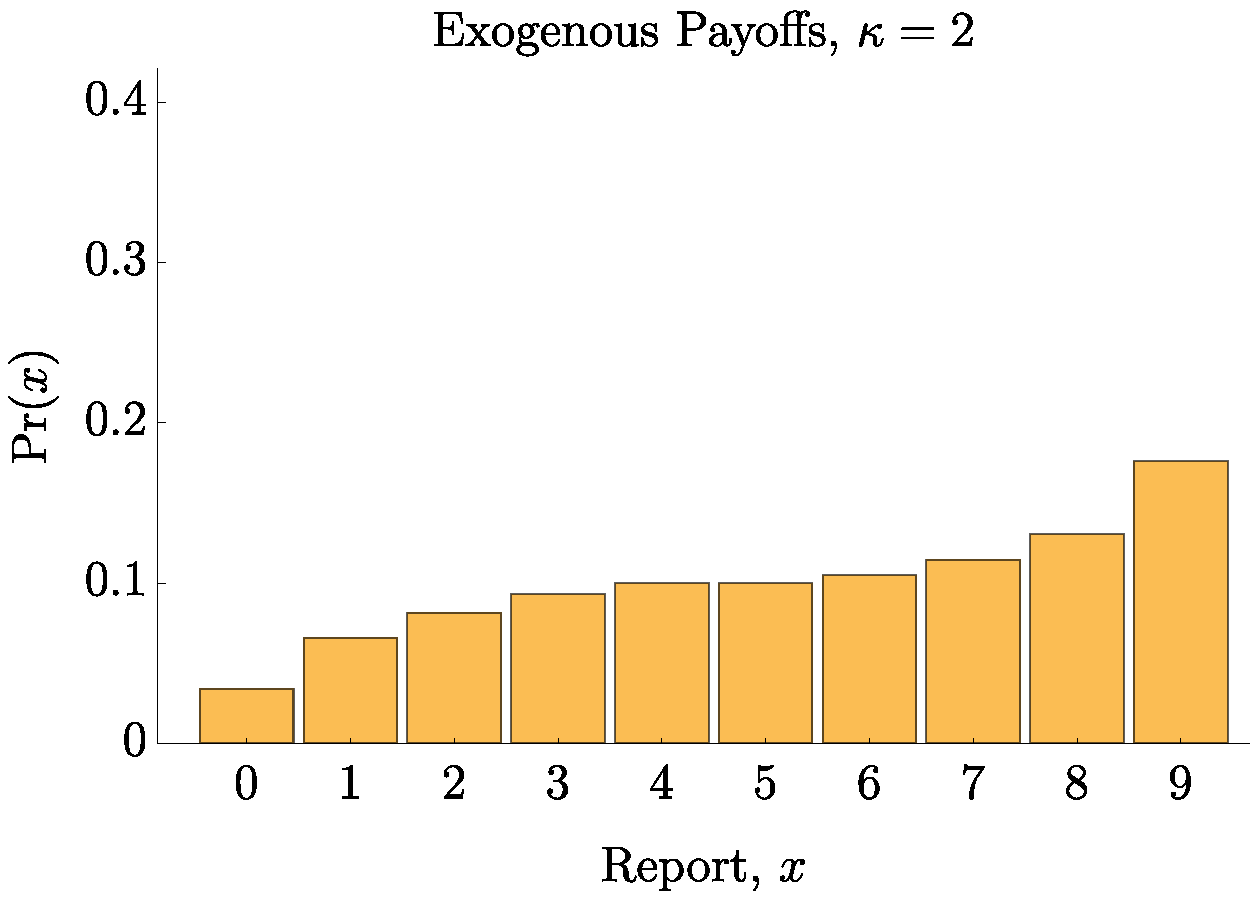
\includegraphics[width=0.49\textwidth]{./ih/pred_hist_ex_2.pdf}
    	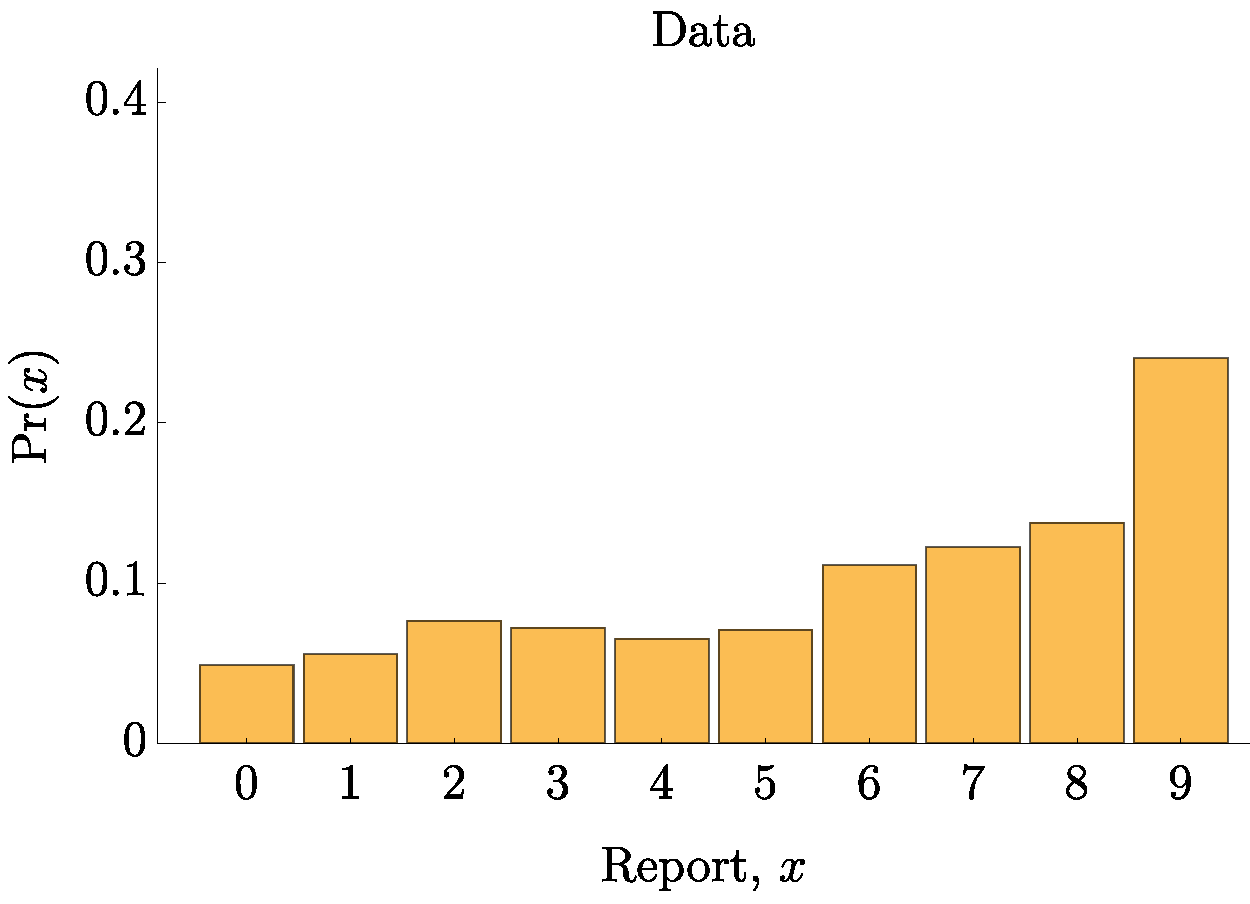
\includegraphics[width=0.49\textwidth]{./ih/emp_hist_ex_nolabel.pdf}
    \end{center}
\end{frame}

\begin{frame}{Questions}
    \begin{eqnarray*}
    U_{i}(\omega,x;\theta) & = & \pi(x)-\boldsymbol{1}_{\omega\not=x}\cdot c-\theta_{i}\cdot\Lambda^{\star}(x)\\
     & \text{} & \text{where},\theta_{i}\sim U[0,\kappa]
    \end{eqnarray*}

    \begin{itemize}
        \item What does the model predict as we endogenize:
            \begin{itemize}
                \item \textbf{Population:} the $\theta$-types that participate: $\Rightarrow\kappa\rightarrow\kappa^{\star}$
                \item \textbf{Payoffs:} the return to each report: $\Rightarrow\pi(x)\rightarrow\pi^{\star}(x)$
                \item \textbf{Both}: $\Rightarrow\left(\kappa,\pi\left(x\right)\right)\rightarrow\left(\kappa^{\star},\pi^{\star}\left(x\right)\right)$
            \end{itemize}
    \end{itemize}
\end{frame}

\begin{frame}{Selection}
    \begin{eqnarray*}
    U_{i}(\omega,x;\theta) & = & \pi(x)-\boldsymbol{1}_{\omega\not=x}\cdot c-\theta_{i}\cdot\Lambda^{\star}(x)\\
     & \text{} & \text{where},\theta_{i}\sim U[0,\kappa]
    \end{eqnarray*}
    
    \begin{itemize}
        \item Fixed setting: given preferences can calculate equilibrium:
            \begin{itemize}
                \item $\xi_{\theta}(\omega)$: action by reputation type $\theta$
                \item $\Lambda^{\star}(x):$ fraction of liars at each report
            \end{itemize}
        \item Provide an outside option $u_{0}$
        \item Ex ante expected payoff is:
        \begin{eqnarray*}
            \mathbb{E}U(\theta) & = & \mathbb{E}U_{i}\left(\omega,\xi_{\theta}\left(\omega\right)\right)\\
         & = & \mathbb{E}\text{Payoff}-c\cdot\text{LyingRate}(\theta)-\theta_{i}\cdot\text{\ensuremath{\mathbb{E}}RepCost}(\theta)
        \end{eqnarray*}
    \end{itemize}
\end{frame}

\begin{frame}{Theory: Expected Payoff by Reputation Cost}
    \begin{center}
        \includegraphics<1>[width=0.9\textwidth]{./ih/ExpectUtilityRep0.pdf}
        \includegraphics<2>[width=0.9\textwidth]{./ih/ExpectUtilityRep1.pdf}
        \includegraphics<3>[width=0.9\textwidth]{./ih/ExpectUtilityRep2.pdf}
    \end{center}
\end{frame}

\begin{frame}{Selection effects}
    \begin{eqnarray*}
    U_{i}(\omega,x;\theta) & = & \pi(x)-\boldsymbol{1}_{\omega\not=x}\cdot c-\theta_{i}\cdot\Lambda^{\star}(x)\\
     & \text{} & \text{where},\theta_{i}\sim U[0,\kappa]
    \end{eqnarray*}

    \begin{itemize}
    \item Self-selection in the model is equivalent to solving for an equilibrium
    $(\xi^{\star},\Lambda^{\star},\kappa^{\star})$
        \begin{itemize}
            \item where $u_{0}=\mathbb{E}U(\kappa^{\star})$
        \end{itemize}
    \end{itemize}
\end{frame}

\begin{frame}{Selection effects}
    \begin{eqnarray*}
        U_{i}(\omega,x;\theta) & = & \pi(x)-\boldsymbol{1}_{\omega\not=x}\cdot c-\theta_{i}\cdot\Lambda^{\star}(x)\\
     & \text{} & \text{where},\theta_{i}\sim U[0,\kappa]
    \end{eqnarray*}
    \begin{itemize}
        \item Self-selection in the model is equivalent to solving for an equilibrium
        $(\xi^{\star},\Lambda^{\star},\kappa^{\star})$
            \begin{itemize}
                \item $u_{0}=H$$,\rightarrow$ $\kappa^{\star}\approx\text{\ensuremath{\min}\{}1,\kappa\}$
                \item $u_{0}=L$$,\rightarrow$ $\kappa^{\star}\approx\text{\ensuremath{\min}\{}5,\kappa\}$
            \end{itemize}
    \end{itemize}
\end{frame}

\begin{frame}{Selection Effects}
    \begin{center}
        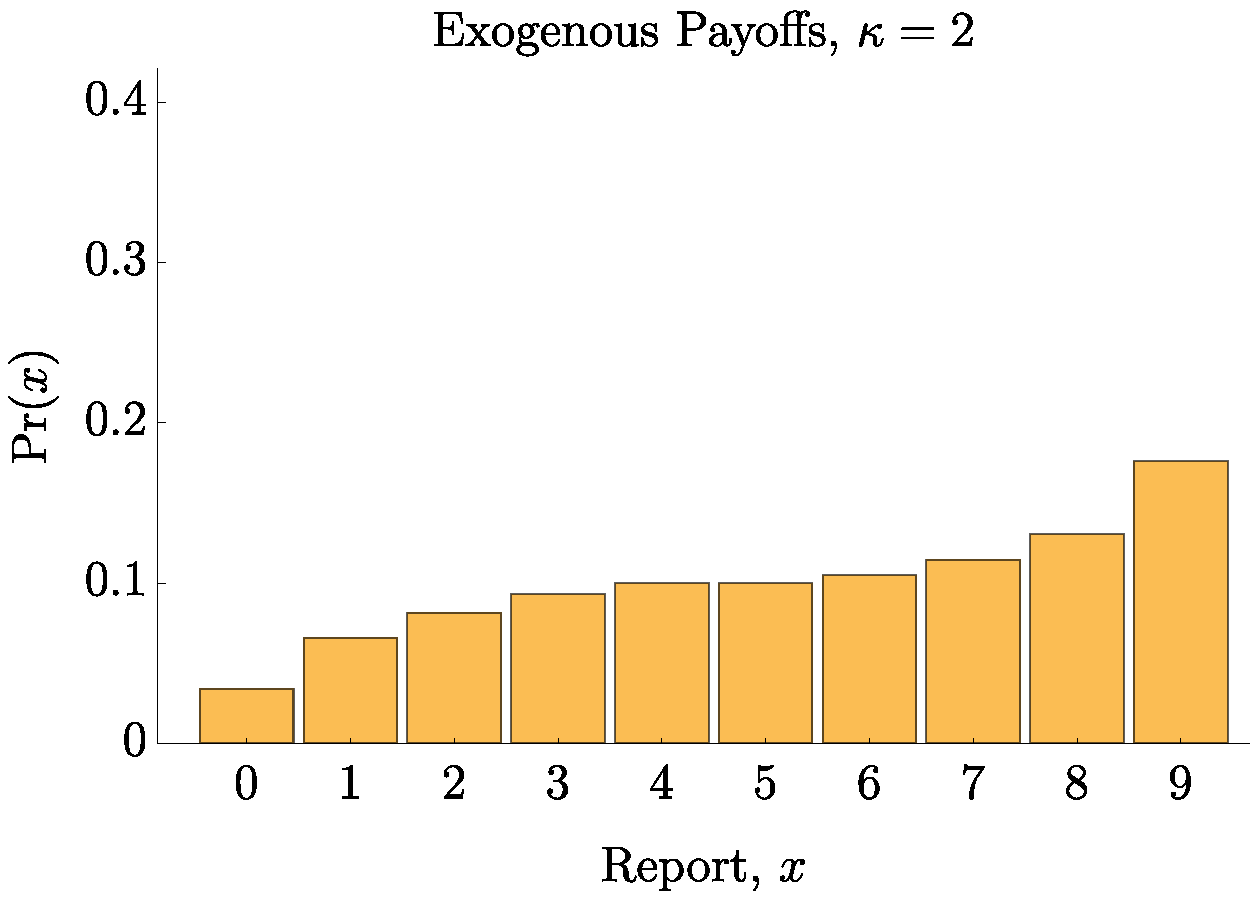
\includegraphics[width=0.4\textwidth]{./ih/pred_hist_ex_2.pdf}
        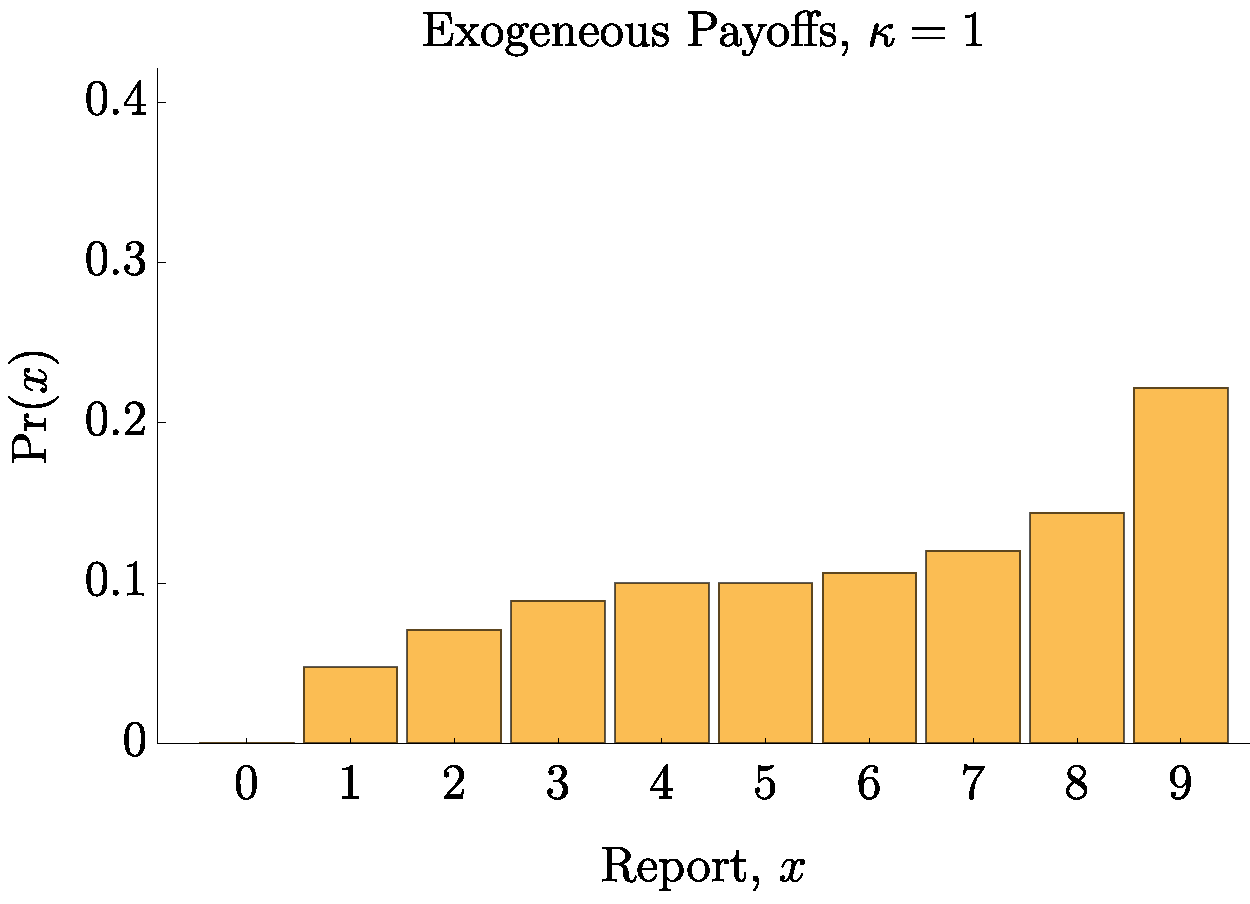
\includegraphics[width=0.4\textwidth]{./ih/pred_hist_ex_1.pdf}
    \end{center}
\end{frame}

\begin{frame}{Competition effects}
    \begin{eqnarray*}
    U_{i}(\omega,x;\theta) & = & \pi^{\star}(x)-\boldsymbol{1}_{\omega\not=x}\cdot c-\theta_{i}\cdot\Lambda^{\star}(x)\\
     & \text{} & \text{where},\theta_{i}\sim U[0,\kappa]
    \end{eqnarray*}

    \begin{itemize}
        \item Endogenizing payoffs through competition shifts payoffs
        \[
        \Pr(x_{i}=\omega_{j})+\Pr(x>\omega_{j})\rightarrow\Pr\left(x=\xi^{\star}(\omega_{j})\right)+\left(x=\xi^{\star}(\omega_{j})\right)
        \]
        \item Competitive payoffs requires us to solve for an equilibrium $(\xi^{\star},\Lambda^{\star},\pi^{\star})$
        \item Main effect is to make\textrm{ $\pi^{\star}(x)$ more convex}
    \end{itemize}
\end{frame}

\begin{frame}{Theory: Endogenizing Payoffs}
    \begin{center}
        \includegraphics<1>[width=0.9\textwidth]{./ih/ExpectUtilityRep3.pdf}
    \end{center}
\end{frame}

\begin{frame}{Theory: Reports}
    \begin{center}
        \includegraphics<1>[width=0.49\textwidth]{./ih/pred_hist_ex_2.pdf}
        \includegraphics<1>[width=0.49\textwidth]{./ih/pred_hist_en_2.pdf}
        \includegraphics<2>[width=0.49\textwidth]{./ih/pred_hist_ex_1.pdf}
        \includegraphics<2>[width=0.49\textwidth]{./ih/pred_hist_en_1.pdf}
        \includegraphics<3>[width=0.49\textwidth]{./ih/pred_hist_ex_half.pdf}
        \includegraphics<3>[width=0.49\textwidth]{./ih/pred_hist_en_half.pdf}
    \end{center}
\end{frame}

\begin{frame}{Broad Predictions}
    \begin{itemize}
        \item Given the meta-study's calibrated parameters and model:
        \item \textbf{Self Selection}:
            \begin{itemize}
                \item Fraction entering decreases in $u_{0}$
                \item Report distribution shifts slightly toward greater dishonesty when
                $u_{0}$ high
            \end{itemize}
        \item \textbf{Endogenous Payoffs}:
            \begin{itemize}
                \item For $\kappa$ large, the shift in reports from exogenous payoffs is
                small
                \item For $\kappa$ small the shifts in reports are much larger
            \end{itemize}
        \item \textbf{Self-Selection and Endogenous Payoffs}
            \begin{itemize}
                \item Large and substantial increases in lying
                \item (Need a richer model with heterogeneity in lying cost $c$)
            \end{itemize}
    \end{itemize}
\end{frame}

\begin{frame}
    \begin{center}
        \textsc{\Huge{}Results}{\Huge\par}
    \end{center}
\end{frame}

\begin{frame}{Entering the Competitive Task}
    \begin{center}
        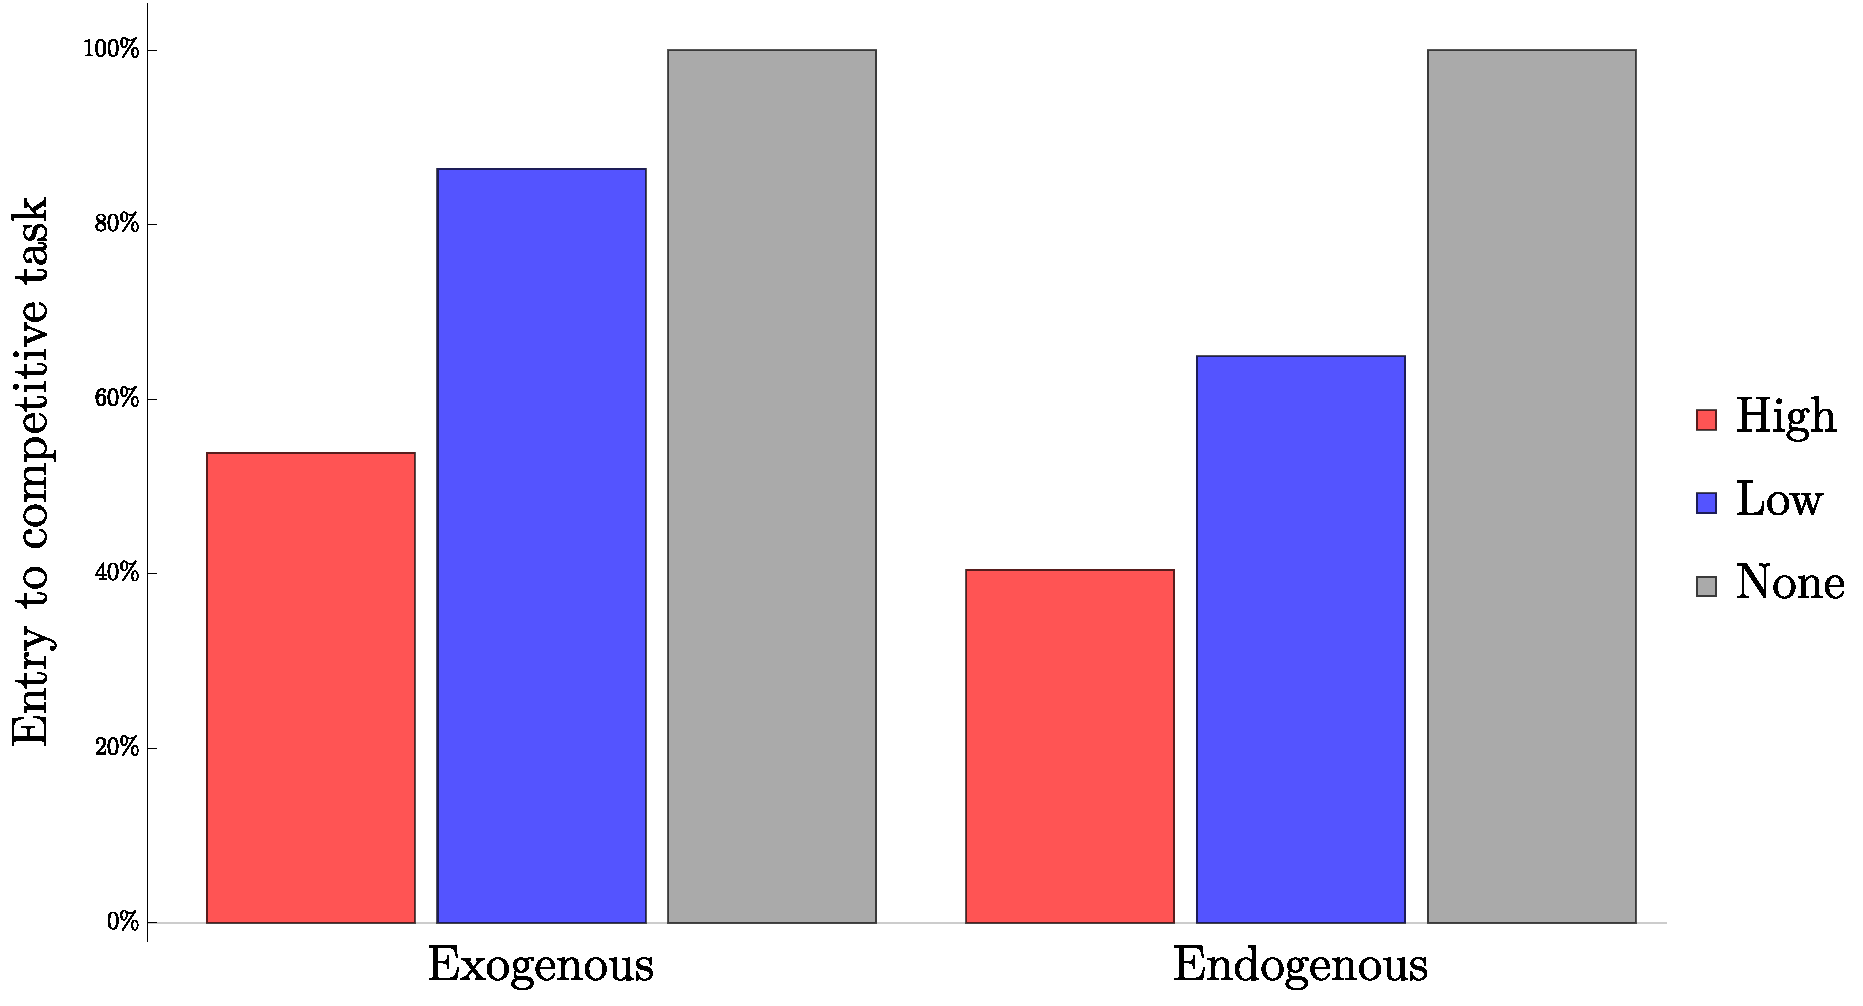
\includegraphics[width=0.8\textwidth]{./ih/col_TaskEntry.pdf}
    \end{center}
\end{frame}

\begin{frame}{Reports: No Outside Option}
    \begin{center}
        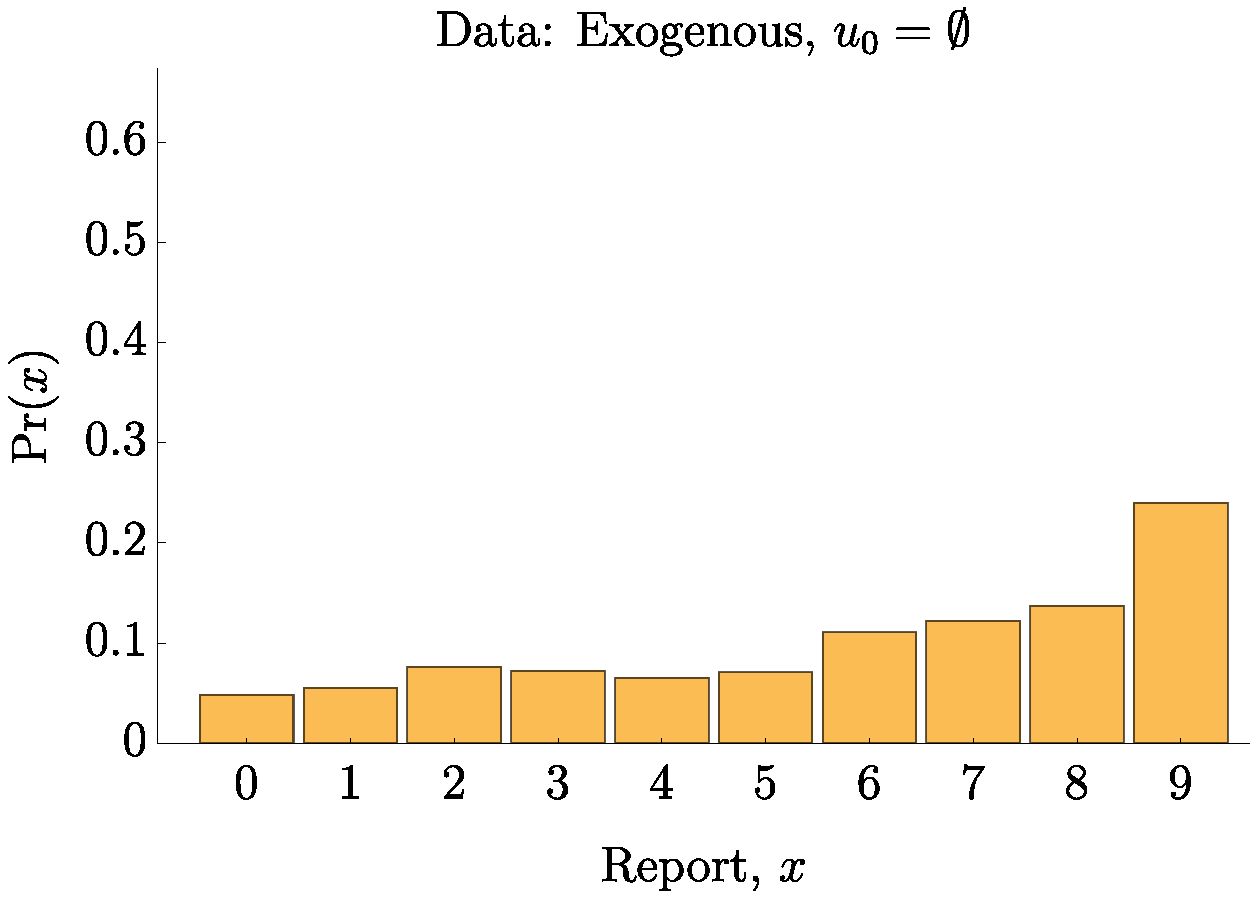
\includegraphics[width=0.5\textwidth]{./ih/emp_hist_ex_none.pdf}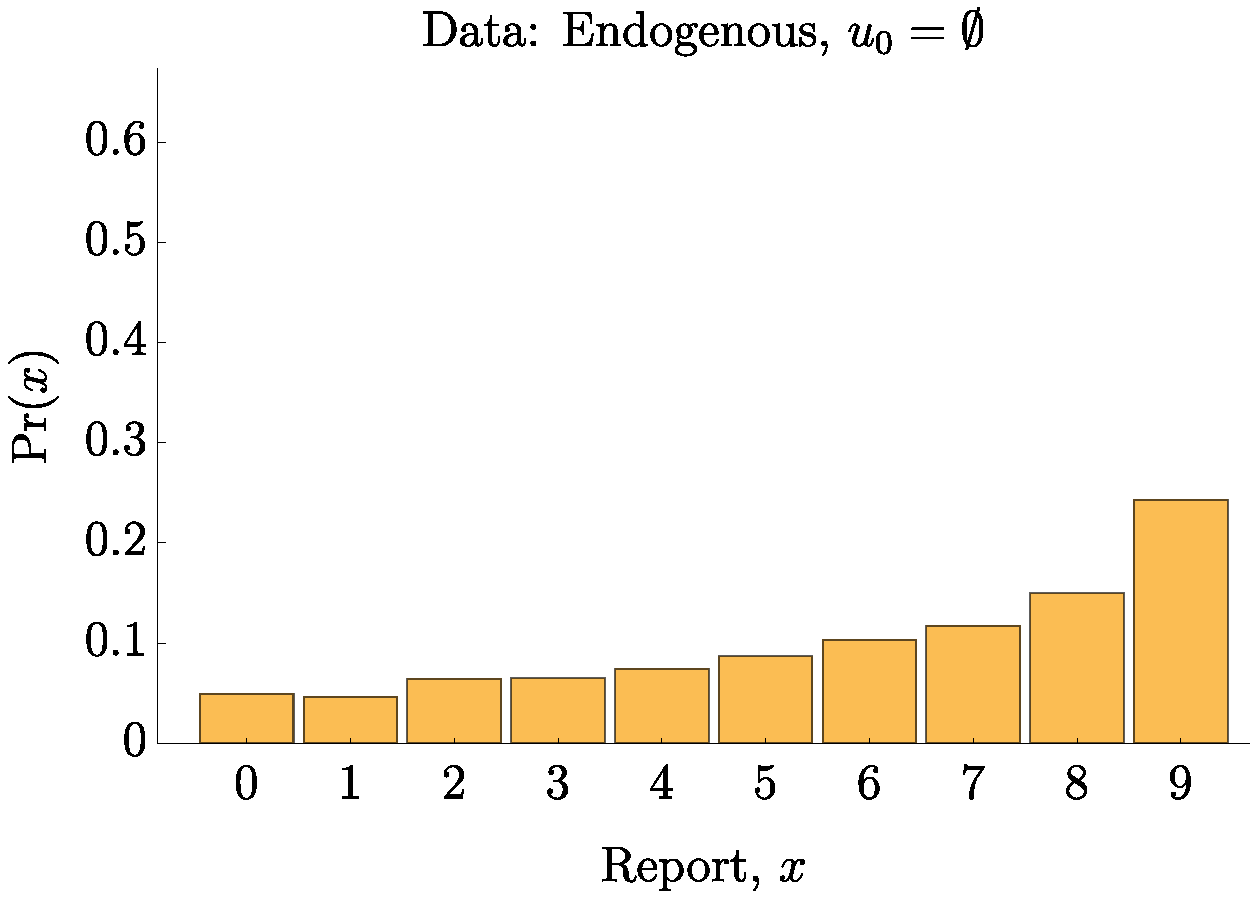
\includegraphics[width=0.5\textwidth]{./ih/emp_hist_en_none.pdf}
    \end{center}
\end{frame}

\begin{frame}{Reports: Exogenous prize}
    \begin{center}
        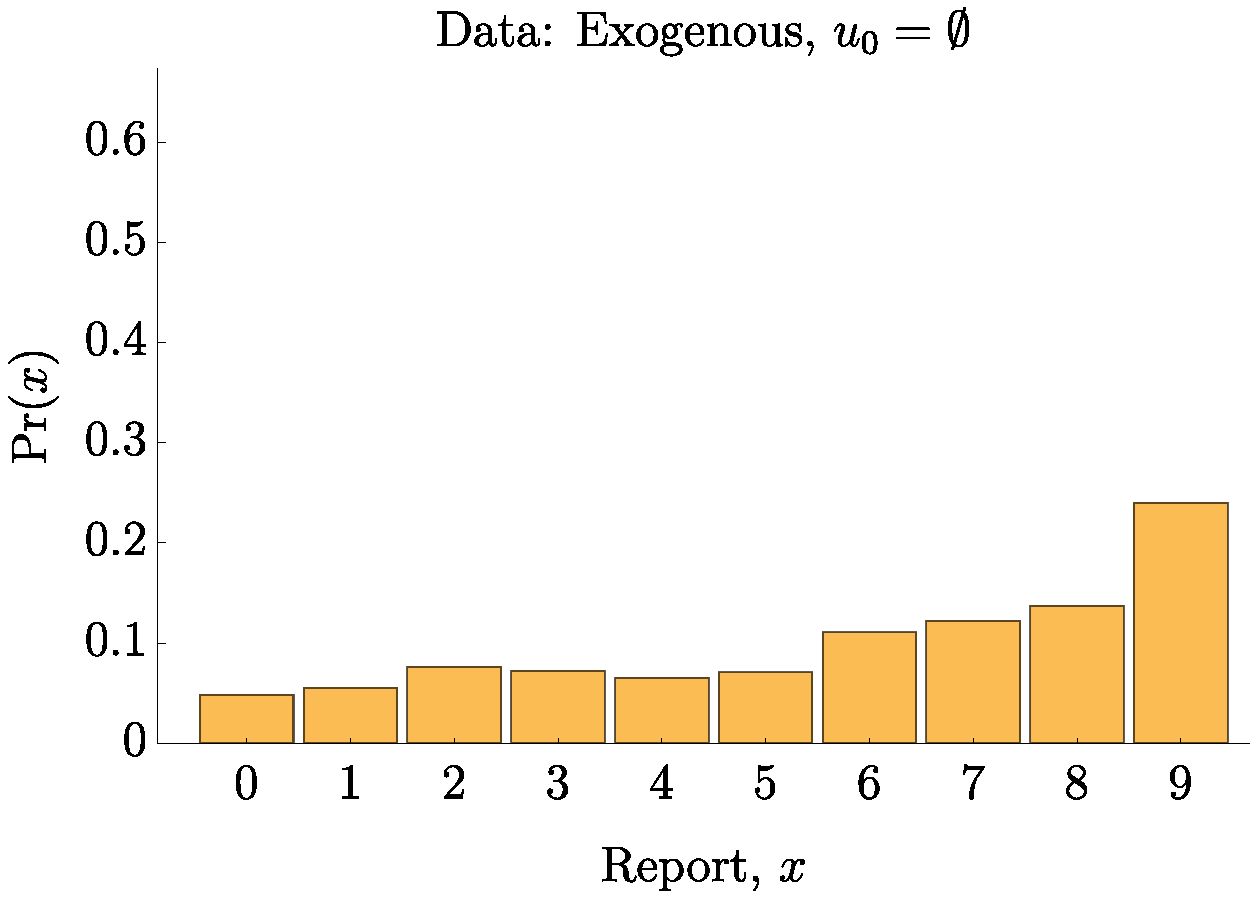
\includegraphics[width=0.32\textwidth]{./ih/emp_hist_ex_none.pdf}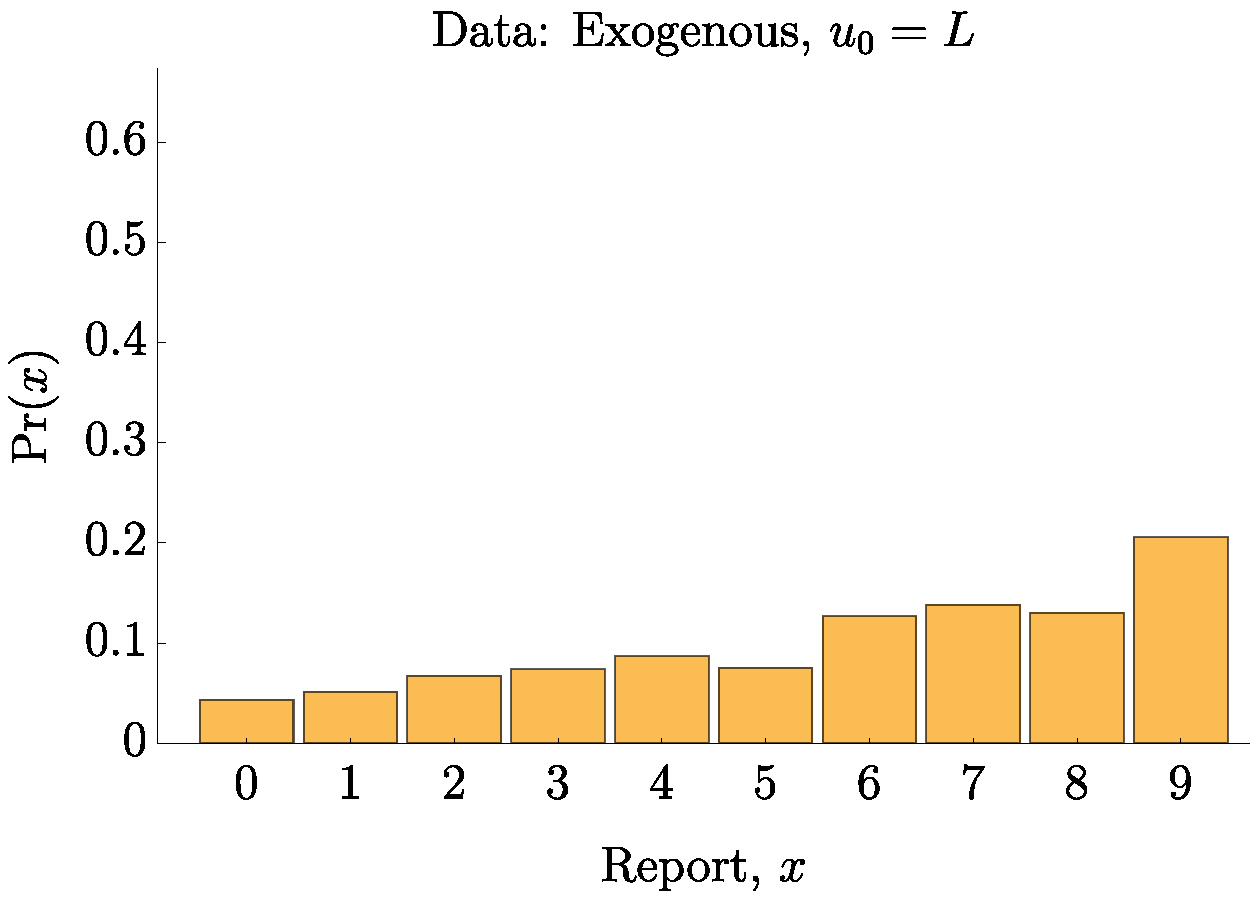
\includegraphics[width=0.32\textwidth]{./ih/emp_hist_ex_L.pdf}
        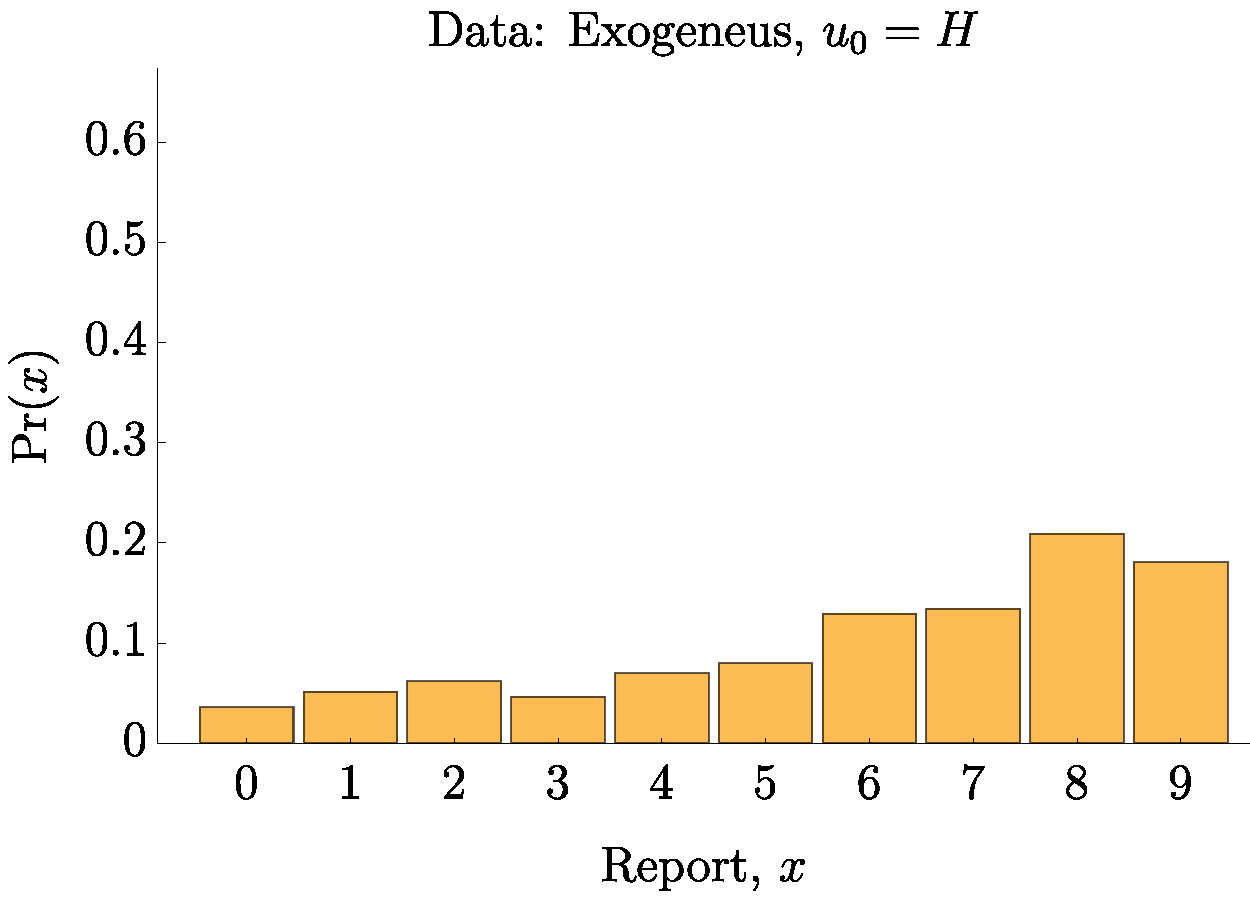
\includegraphics[width=0.32\textwidth]{./ih/emp_hist_ex_H.pdf}
    \end{center}
\end{frame}

\begin{frame}{Reports: Both}
    \begin{center}
        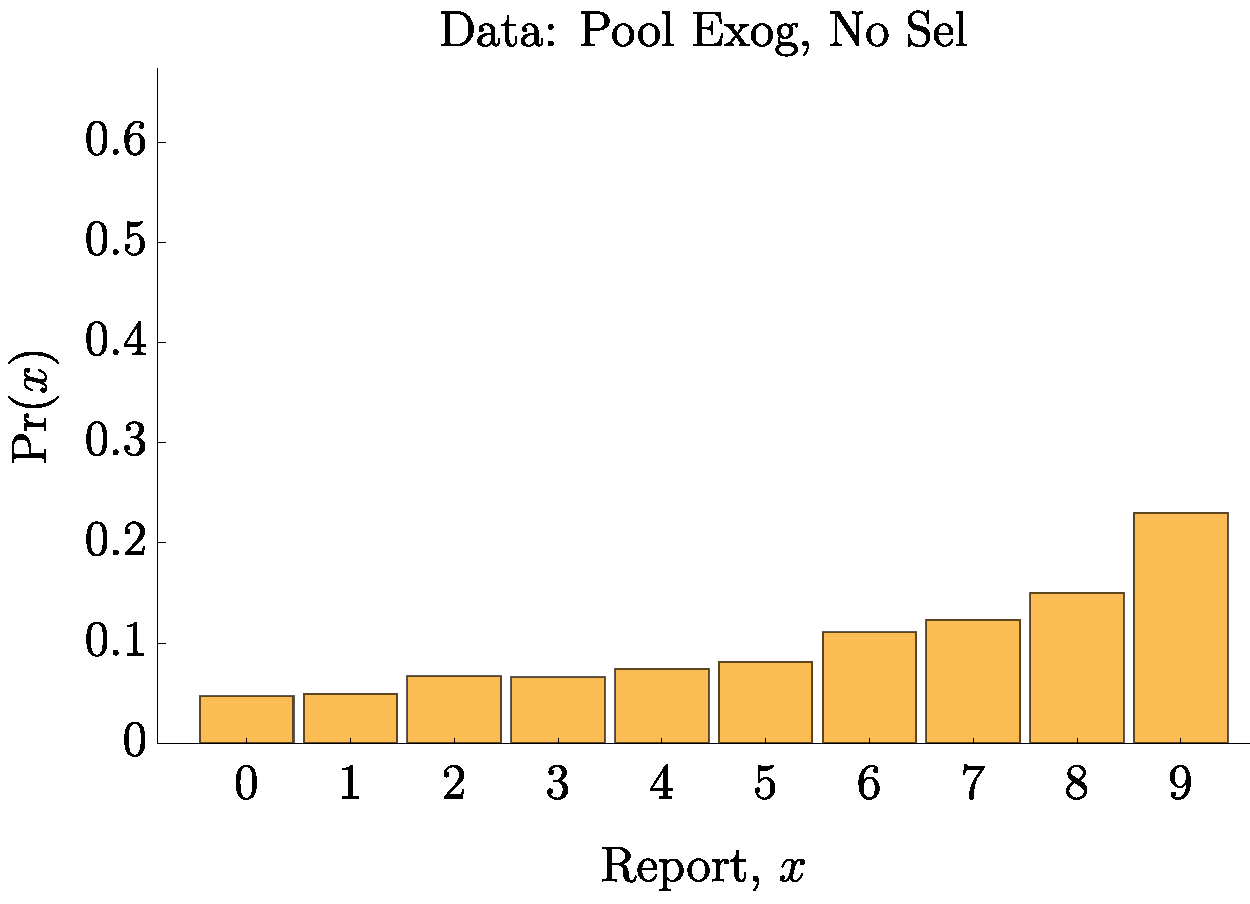
\includegraphics[width=0.32\textwidth]{./ih/emp_hist_pool.pdf}
        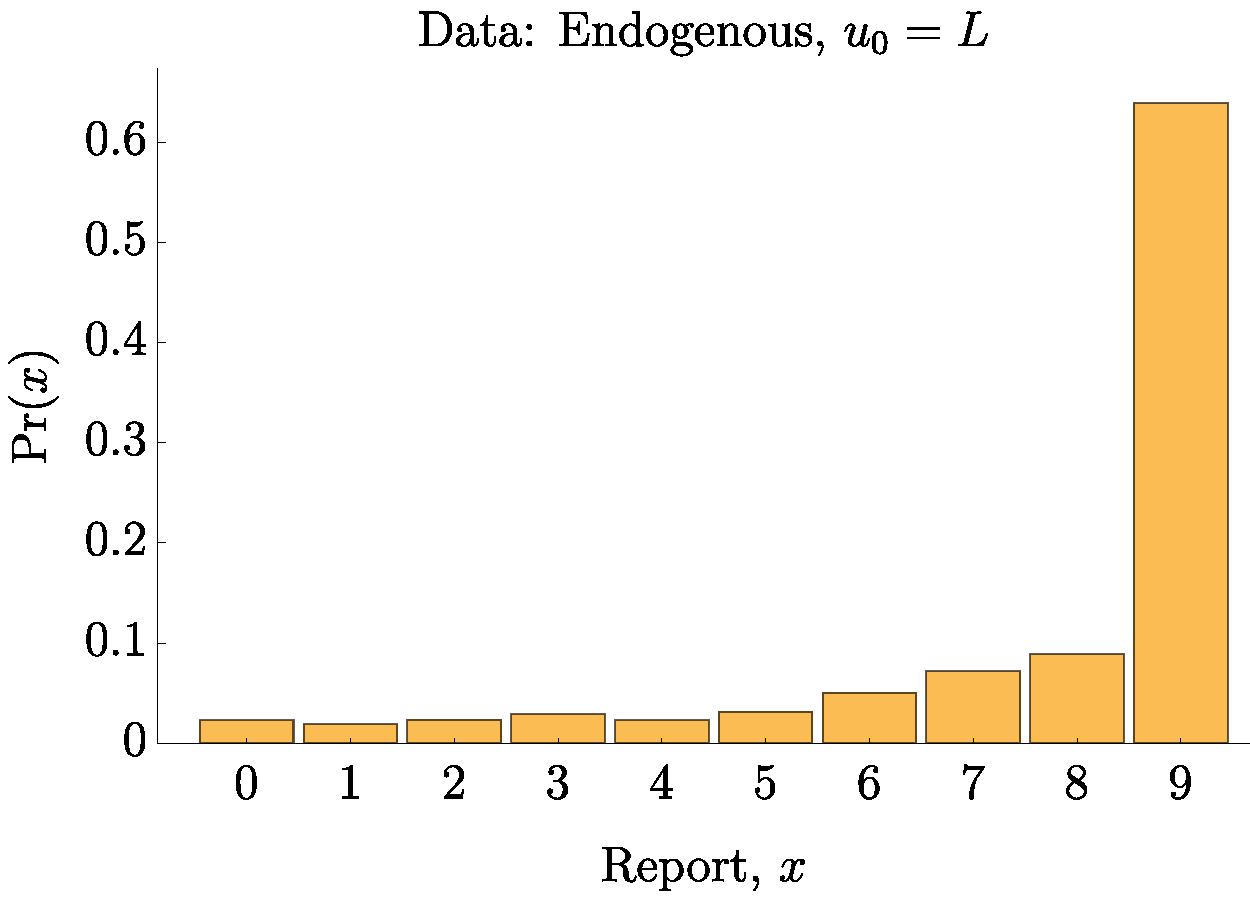
\includegraphics[width=0.32\textwidth]{./ih/emp_hist_en_L.pdf}
        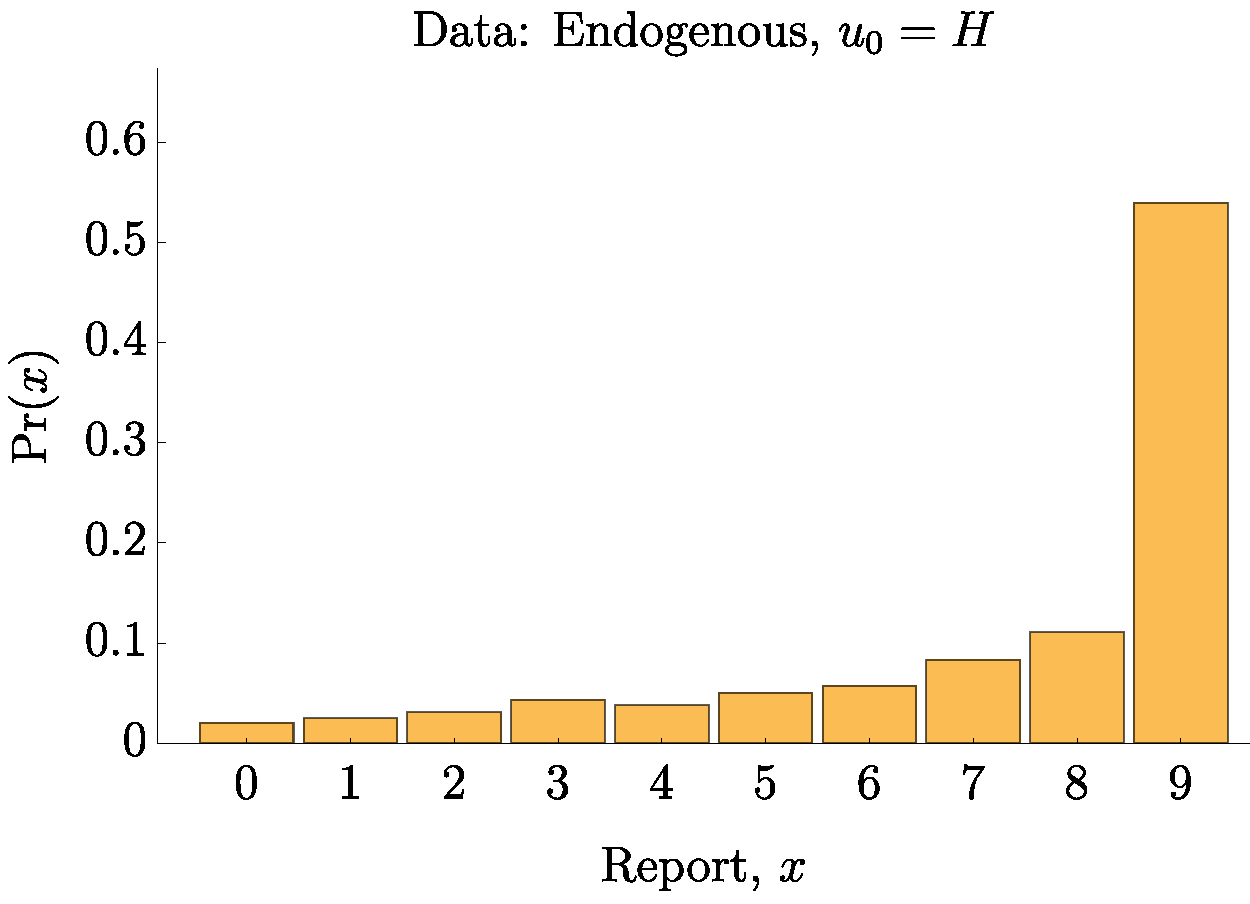
\includegraphics[width=0.32\textwidth]{./ih/emp_hist_en_H.pdf}
    \end{center}
\end{frame}

\begin{frame}{Results}
    \begin{center}
        \begin{tabular}{cccccccc}
        \toprule \textbf{Variable} & \multicolumn{3}{c}{\textbf{Exog-$\pi$}} &  & \multicolumn{3}{c}{\textbf{Endog-$\pi^{\star}$}}\\ 
        \cmidrule{2-4}\cmidrule{6-8} & \textbf{$\emptyset$} & \textbf{L} & \textbf{H} &  & \textbf{$\emptyset$} & \textbf{L} & \textbf{H}\\ 
        \midrule \textbf{Entry Rate} & 1 & 0.86 & 0.54 &  & 1 & 0.65 & 0.40\\ 
        \textbf{Fixed Report} & \textendash{} & 4.52 & 4.52 &  & \textendash{} & 4.72 & 4.58\\ 
        \textbf{Comp. Report} & 5.82 & 5.76 & 6.01 &  & 5.92 & 7.68 & 7.29\\ 
        \bottomrule
        \end{tabular}
    \end{center}
\end{frame}

\begin{frame}{Results}
    \begin{center}
        \begin{tabular}{cccccccc}
        \toprule \textbf{Variable} & \multicolumn{3}{c}{\textbf{Exog-$\pi$}} &  & \multicolumn{3}{c}{\textbf{Endog-$\pi^{\star}$}}\\ 
        \cmidrule{2-4}\cmidrule{6-8} & \textbf{$\emptyset$} & \textbf{L} & \textbf{H} &  & \textbf{$\emptyset$} & \textbf{L} & \textbf{H}\\ 
        \midrule \textbf{Entry Rate} & 1 & 0.86 & 0.54 &  & 1 & 0.65 & 0.40\\ 
        \textbf{Fixed Honesty} & \textendash{} & 1.00 & 1.00 &  & \textendash{} & 0.95 & 0.98\\ 
        \textbf{Comp. Honesty} & 0.71 & 0.72 & 0.66 &  & 0.68 & 0.29 & 0.38\\ 
        \bottomrule  &  &  &  &  &  &  & \\ 
        \end{tabular}
    \end{center}

Transform average reports to ``implied honesty'' via following:
\[
x\mapsto(9-x)/4.5
\]
\end{frame}

\begin{frame}{Results--Comparative Statics}
    \begin{center}
        \begin{tabular}{ccc}
        \toprule \textbf{Variable} & \multicolumn{2}{c}{\textbf{Joint Tests}}\\ 
        \cmidrule{2-3}  & $\boldsymbol{Ex}$ vs. $\boldsymbol{En}$ & \textbf{$\emptyset$} vs. $\boldsymbol{L}$ vs. $\boldsymbol{H}$\\ 
        \midrule \textbf{Entry Rate} & $\boldsymbol{Ex}{\color{red}\stackrel{\star\star\star}{\succ}}En$ & $\boldsymbol{L}{\color{red}\stackrel{\star\star\star}{\succ}}\boldsymbol{H}$\\ 
        \textbf{Fixed Honesty} & $\boldsymbol{Ex}\sim\boldsymbol{En}$ & $\boldsymbol{L}\sim\boldsymbol{H}$\\ 
        \textbf{Comp. Honesty} & $Ex{\color{red}\stackrel{\star\star\star}{\succ}}En$ & $\boldsymbol{\emptyset}{\color{red}\stackrel{\star\star\star}{\succ}}\boldsymbol{L}\sim\boldsymbol{H}$\\ 
        \bottomrule  &  & \\ 
        \end{tabular}
    \end{center}
\end{frame}

\begin{frame}{Aggregate Result}\begin{center}

\textbf{Result: }The interaction of selection with endogenous payoffs
substantially reduces honest revelation, with minimal effects from
each separate term.
\end{center}

\[
\hat{\lambda}=\underset{(0.062)}{0.706}-\underset{(0.076)}{0.007}\cdot\text{Sel}-\underset{(0.072)}{0.023}\cdot\text{En-}\ensuremath{\pi}-\underset{(0.090)}{0.349}\cdot\text{Sel\ensuremath{\times\text{En-\ensuremath{\pi}}.}}
\]
\end{frame}

\begin{frame}{Subject-level calculation}
    \begin{itemize}
        \item Above we looked at aggregate data, can instead look at the subject
        level
        \item For each subject with at least 5 rounds in the competitive task, we
        calculate their implied honesty:
            \begin{itemize}
                \item $\lambda_{i}=\frac{2}{9}\left(9-\frac{1}{\#Comp.}\sum x_{it}^{\text{Comp}}\right)$
                \item Then look at the smoothed distribution of $\lambda_{i}$
            \end{itemize}
    \end{itemize}
\end{frame}

\begin{frame}{Subject average honesty}
    \begin{center}
    	\includegraphics<1>[width=0.9\textwidth]{./ih/col_indivHonesty.pdf}
    \end{center}
\end{frame}

\begin{frame}{Group Dynamics}
    \begin{center}
    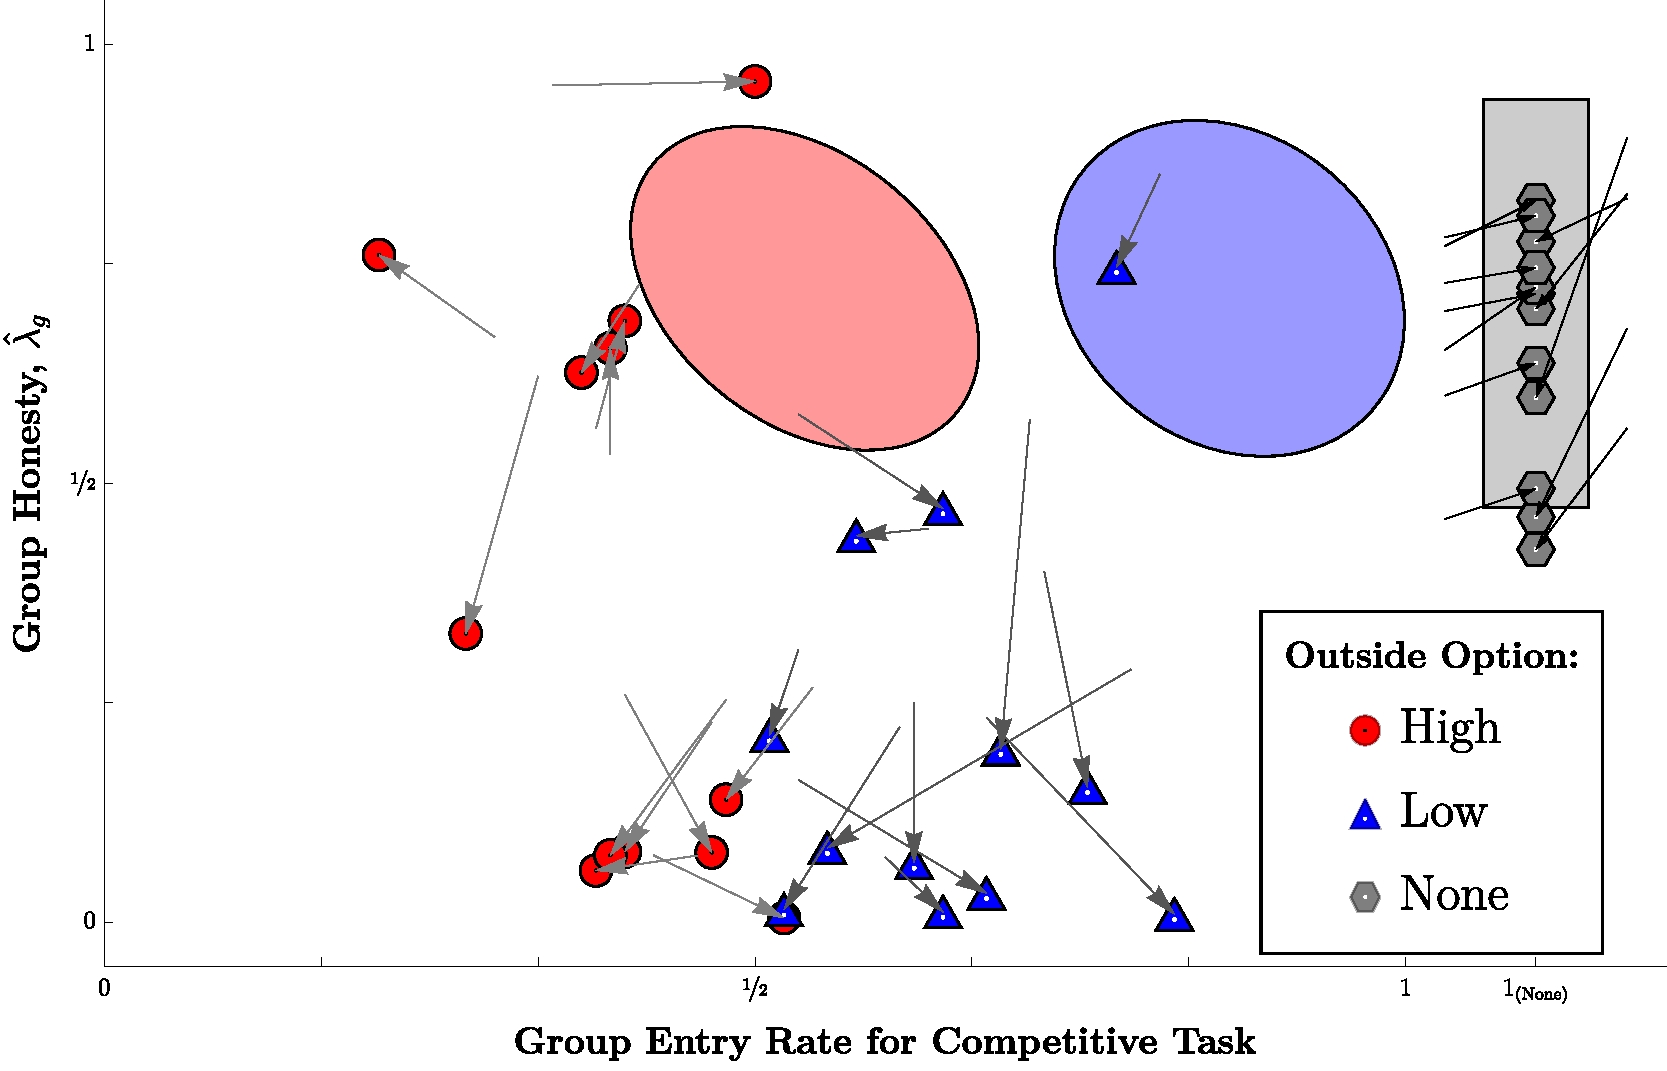
\includegraphics[width=0.8\textwidth]{./ih/col_Scatter_Group_WithArrowsEllipse.pdf}
    \end{center}
\end{frame}


\begin{frame}{Conclusions}
    \begin{itemize}
        \item Look at a repeated honesty task with task selection and competition
        \item Without \textbf{both} selection and prize endogeneity, our task leads
        to very similar results to the standard literature
        \item With \textbf{both} aggregate responses are much closer to the payoff-maximizing
        predictions
        \item Heterogeneity in the group results suggests a critical threshold below
        which our matching groups spiral down towards complete dishonesty
            \begin{itemize}
                \item Smaller communities more bi-modal
            \end{itemize}
        \item Reputational models do well at helping us understand the data across
        treatments
            % \begin{itemize}
            %     \item That said, they're computationally very complex
            % \end{itemize}
    \end{itemize}
\end{frame}

\end{document}
